\documentclass[11pt]{article}

\usepackage[T1]{fontenc}
\usepackage[utf8]{inputenc}
\usepackage[margin=1in]{geometry}
\usepackage{amsmath,amssymb,amsthm,mathtools}
\usepackage{booktabs}
\usepackage{graphicx}
\usepackage{microtype}
\usepackage{natbib}
\usepackage{xcolor}
\usepackage{enumitem}
\usepackage{hyperref}
\hypersetup{colorlinks=true,linkcolor=blue!55!black,citecolor=blue!55!black,urlcolor=blue!55!black}

\newtheorem{theorem}{Theorem}
\newtheorem{proposition}[theorem]{Proposition}
\newtheorem{lemma}[theorem]{Lemma}
\newtheorem{corollary}[theorem]{Corollary}
\theoremstyle{definition}
\newtheorem{definition}[theorem]{Definition}
\theoremstyle{remark}
\newtheorem{remark}[theorem]{Remark}

\newcommand{\R}{\mathbb R}
\newcommand{\E}{\mathbb E}
\newcommand{\cL}{\mathcal L}
\newcommand{\cB}{\mathcal B}
\newcommand{\cX}{\mathcal X}
\newcommand{\ip}[2]{\left\langle #1,#2\right\rangle}
\newcommand{\norm}[1]{\left\lVert #1\right\rVert}
\newcommand{\od}{\mathop{}\!\mathrm d}
\newcommand{\what}{\widehat}
\newcommand{\Pproj}{\Pi}

\title{Compressing Neural Training Dynamics with Response Memory}
\author{Anonymous working-paper draft}
\date{September 2026}

\begin{document}
\maketitle

\begin{abstract}
Compressing a trained network at one time does not by itself compress its
training dynamics: two functionally identical states can respond differently
to the next gradient update, and small local errors can accumulate through
feedback.  We study this problem for fixed-depth, fully connected nonlinear
networks under feature-learning gradient-flow scaling.  Every learned hidden
matrix is the initialized matrix plus a time integral of outer products of a
forward response and a backward response.  We replace the growing response
history by a fixed number $P$ of evolving shifted-Legendre moments per neuron,
sample, and internal layer.  The moments form an autonomous closure, while the
initialized matrices and their transposes are retained exactly.

For arbitrary fixed width, dataset, depth, initialization, and finite time
horizon, we prove uniform tracking of dense gradient flow.  A residual-activity
clock gives physical-state error $O(P^{-1})$ for locally $C^{1,1}$ activations.
A response-arclength clock controls the joint forward/backward path and gives
$O(P^{-2})$ for the corresponding smoother activation class.  These are
global finite-horizon results: the horizon is arbitrary but the constants are
not uniform over infinite training time or width.  The closure compresses the
learned moving correction to $O(nmP)$ coordinates per internal layer and rank
at most $mP$ (or $m(P+1)$ for the weighted clock), but it retains $O(n^2)$
initialized operators and their dense actions.  It is therefore a compression
of learned moving state, not yet a compression of the whole model.

Finite experiments support the construction.  On five sparse-label circle
tasks at width 2048, order seven reproduces the dense fitted function with
RMS discrepancies from about $4\times10^{-6}$ to $4.7\times10^{-3}$.  On a
width-4096 MNIST 3-versus-8 experiment with 100 training images, orders one
through three agree with dense predictions on 1984 held-out images to RMS
$3.25\times10^{-3}$, $1.08\times10^{-3}$, and $1.20\times10^{-3}$.  Broader
tests also expose low-order failures and show that the sharper clock is not
uniformly better at practical orders.  We give exact complexity accounting,
state the population-limit interpretation that is currently justified, and
separate it from the still-open width-uniform compression problem.
\end{abstract}

\section{Why training compression is different}
\label{sec:introduction}

The primary question of this paper is simple:
\emph{how much can one compress the training dynamics of a neural network?}
The analogous question for a single trained snapshot is much easier to pose.
One may prune or factor its weights, distill its predictions, or approximate
its input--output map.  None of these operations alone supplies a compressed
state for continued training.  Two parameter states can represent the same
function on every input and still have different tangent features.  Their
next gradient updates can therefore differ.  A small one-step discrepancy can
then feed back into later activations, gradients, and updates.

We call a compression of training \emph{global on finite horizons} if, for
each finite $T$ and tolerance $\varepsilon$, one can choose a finite
compression order so that one autonomous compressed trajectory stays within
$\varepsilon$ of the dense trajectory for every $0\le t\le T$.  This is
stronger than approximating the vector field at one state and weaker than a
single error bound uniform over $0\le t<\infty$.  The state dimension should
remain constant as elapsed training time grows.  It may still depend on the
requested accuracy, dataset size, depth, and the representation class.

This question is scientifically useful even before it produces a smaller
implementation.  An accurate autonomous compression identifies information
that is sufficient for future learning, not merely for current prediction.
It can expose which aspects of the dense trajectory carry memory and which
details may be discarded.  Our nonnegotiable target retains three ingredients
together: more than one hidden layer, nonlinear responses that remain active,
and feature learning rather than a fixed-kernel linearization.

Wide-network limits offer a natural setting for this program.  With an
appropriate maximal-update or mean-field scaling, nontrivial feature motion
survives at large width \citep{yang2021tensor,nguyen2023rigorous}.  Empirical
averages may converge to deterministic fields, much as particle systems lead
to continuum descriptions.  Existing tensor-program, mean-field, and
dynamical-field theories provide powerful exact descriptions of such limits
\citep{yang2021tensor,nguyen2023rigorous,bordelon2022selfconsistent}.  In the
deep feature-learning settings closest to ours, however, exact descriptions
retain operators, two-time kernels, or a growing family of historical
responses.  They do not by themselves show that the learned dynamics can be
approximated by a fixed amount of history state throughout training.

The observation behind our construction is elementary.  For every internal
layer, gradient flow writes the learned matrix increment as an integral of
rank-one products,
\begin{equation}
 W_\ell(t)-W_{\ell,0}
 =-\frac{2}{nm}\sum_{a=1}^{m}\int_0^t
 r_a(s)\,\delta_{\ell,a}(s)h_{\ell-1,a}(s)^\top\,\od s .
 \label{eq:intro-history}
\end{equation}
Exact history storage grows with time.  We instead project the forward and
backward response paths onto the first $P$ shifted Legendre modes and evolve
their coefficients online.  The closure reconstructs the learned interaction
from these moment pairs.  Shifted Legendre memory is closely related to the
online polynomial-projection principle developed by HiPPO
\citep{gu2020hippo}.  The contribution here is to couple such memory to the
forward/backward feedback of deep gradient flow, preserve the reused
initialized operator in both orientations, and prove trajectory tracking for
the resulting autonomous nonlinear closure.

Two clocks produce two guarantees.  The first advances at residual RMS.  It
removes the residual factor from forward response speed and gives an
$O(P^{-1})$ state bound at arbitrary fixed depth.  The second advances at
residual activity plus the arclength of all stored forward and backward
responses.  It also keeps the original learning measure inside the history
integral.  Both histories then have first-order projection error, and their
outer-product error is $O(P^{-2})$.

The main contributions are as follows.
\begin{enumerate}[leftmargin=*,itemsep=0.35em]
\item We give explicit autonomous response-memory ODEs for a fixed number of
      moments per neuron, sample, and internal layer.  They retain each
      initialized matrix $W_{\ell,0}$ and its transpose exactly and never use
      a dense reference trajectory.
\item For arbitrary fixed width, finite dataset, fixed depth, arbitrary finite
      initialization, and any prescribed finite horizon, we prove uniform
      dense-trajectory error $O(P^{-1})$ for the activity clock and
      $O(P^{-2})$ for the response clock.  The proof controls the closure's
      own nonlinear feedback by an exact accumulator identity and a first-exit
      argument.
\item We distinguish three representation classes---scalar, population, and
      operator dynamics---and record a restricted exact scalar nonclosure
      theorem.  The response closure compresses the learned state to
      population fields but remains a hybrid with fixed initialized operators.
\item We give complete state, rank, and per-step cost accounting.  The learned
      correction has $O(nmP)$ moving coordinates per internal layer, while the
      exact initialized operators still require $O(n^2)$ storage and dense
      actions.  No total-model or generic runtime improvement is claimed.
\item We test the construction on sparse circle tasks, deeper networks,
      several activations, sphere tasks, and MNIST.  The experiments show high
      fidelity at small order in many cases, together with order reversals,
      numerical sensitivity, and difficult cases where low order fails.
\end{enumerate}

The distinction between proved and prospective population claims matters.
The central approximation theorem in this paper is pathwise at fixed finite
width.  Combining it with a separately established population limit gives a
diagonal sequence of closure orders converging to the same population
observables.  We do not prove that one fixed order works uniformly in width,
or that the closure constants remain controlled for all training time.

\section{Problem, model, and representation classes}
\label{sec:problem}

\subsection{Three meanings of a finite dynamical description}

The word \emph{finite} hides substantial differences.  We use the following
classification.

\begin{definition}[Scalar, population, and operator state]
A \emph{scalar ODE} has state in $\R^q$ for fixed $q$.  A
\emph{population ODE} has a fixed finite list of scalar or vector fields on
fixed probability spaces; an $n$-particle discretization stores one value per
particle and field.  An \emph{operator ODE} has a fixed finite list of
operators between population spaces.  Such an operator can retain arbitrary
row--column correlations and is generally not specified by finitely many
population fields or scalars.
\end{definition}

Counting only the number of named objects would call all three descriptions
finite, but their information content is different.  A general limiting
operator is the continuum analogue of a dense matrix.  Likewise, one
unrestricted field can encode an arbitrary amount of information in its
spatial profile.  Any compression statement must therefore name both the
number and the type of retained objects.

Our closure is a finite collection of neuron-population fields indexed by
sample, layer, and history mode, together with fixed initialized operators.
The learned moving part is population-valued; the total representation is a
population/operator hybrid.  At finite width these fields are simply neuron
vectors.

Exact finite scalar closure is already obstructed in a broad natural class.
The following result is included to calibrate the target, not to claim an
impossibility theorem for every conceivable encoder.

\begin{proposition}[Restricted exact scalar nonclosure]
\label{prop:scalar-no-go}
Consider a state-universal deep linear feature-learning system with several
trainable factors.  Suppose an encoder consists of a fixed finite list of
complete tensor contractions whose connected graph degree is bounded
independently of width, its dynamics are a width-independent polynomial ODE,
and the output is a polynomial readout.  No such encoder exactly realizes the
output dynamics on a nonempty open set for all sufficiently large widths.
The same conclusion holds for analytic finite-jet closures near the zero
state.  It does not rule out arbitrary encoders or a closure restricted to one
initialized trajectory.
\end{proposition}

The proof, given in Appendix~\ref{app:scalar-no-go}, repeatedly differentiates
the output.  It produces connected contractions of unbounded graph degree,
whereas polynomial operations on a fixed bounded-degree alphabet can only
form disjoint unions of its existing connected components.  Stable graph
independence at large width makes the contradiction algebraic.  This result
motivates approximate population memory; it does not prove that every exact
scalar compression is impossible.

\subsection{Deep nonlinear feature-learning gradient flow}

Fix input dimension $d$, sample count $m$, width $n$, and $L\ge2$ hidden
layers.  The data are $(x_a,y_a)_{a=1}^m$ and $u_a=x_a/\sqrt d$.  Hidden
layers have common width only to simplify notation.  With coordinatewise
activations $\phi_\ell$,
\begin{align}
z_{1,a}&=W_1u_a, & h_{1,a}&=\phi_1(z_{1,a}),\nonumber\\
z_{\ell,a}&=W_\ell h_{\ell-1,a}, &
h_{\ell,a}&=\phi_\ell(z_{\ell,a}),\qquad 2\le\ell\le L,\label{eq:model-forward}\\
f_a&=\frac1n w^\top h_{L,a}, & r_a&=f_a-y_a .\nonumber
\end{align}
Here $W_1\in\R^{n\times d}$, $W_\ell\in\R^{n\times n}$ for
$2\le\ell\le L$, and $w\in\R^n$.  We use unhalved mean squared loss
\begin{equation}
 \cL=\rho^2,\qquad
 \rho=\left(\frac1m\sum_{a=1}^m r_a^2\right)^{1/2}.
 \label{eq:loss}
\end{equation}
Backpropagated response fields omit the loss derivative:
\begin{align}
\delta_{L,a}&=w\odot\phi_L'(z_{L,a}),\nonumber\\
\delta_{\ell,a}&=\phi_\ell'(z_{\ell,a})\odot
 W_{\ell+1}^\top\delta_{\ell+1,a},\qquad \ell<L .
\label{eq:backward}
\end{align}

The block mobilities $(n,1,\ldots,1,n)$ are the canonical
feature-learning scaling used throughout the paper.  The resulting gradient
flow is
\begin{align}
\dot W_1&=-\frac2m\sum_a r_a\delta_{1,a}u_a^\top,\nonumber\\
\dot W_\ell&=-\frac{2}{nm}\sum_a
 r_a\delta_{\ell,a}h_{\ell-1,a}^\top,
 \qquad 2\le\ell\le L,\label{eq:dense-gf}\\
\dot w&=-\frac2m\sum_a r_a h_{L,a}.\nonumber
\end{align}
All layers move at order one under the intended wide scaling, so the model is
not reduced to a frozen neural tangent kernel \citep{jacot2018ntk,yang2021tensor}.

Let $\theta=(W_1,\ldots,W_L,w)$ and denote the right-hand side of
\eqref{eq:dense-gf} by $F(\theta)$.  Integrating an internal-layer equation
gives \eqref{eq:intro-history}.  Define, when $\rho>0$,
\begin{equation}
 b_{\ell,a}=\frac{r_a\delta_{\ell,a}}{\rho}.
 \label{eq:b-definition}
\end{equation}
Then the learned increment is the integral of $b_{\ell,a}h_{\ell-1,a}^\top$
against activity measure $\rho(t)\od t$.  The closure will compress exactly
these paired histories.

\subsection{Why the population regime remains the target}

Under Gaussian or sub-Gaussian initialization, fixed depth and data, and
globally Lipschitz activation derivatives, established multilayer mean-field
theorems construct nonlinear population flows on a common local interval and
identify finite-network observables as width grows
\citep{nguyen2023rigorous}.  Maximal-update tensor programs likewise identify
feature-learning limits for discrete training \citep{yang2021tensor}.  These
results justify studying a deterministic population target rather than only
one finite random network.

The following specialized background statement records the population result
used to motivate this paper's regime.

\begin{proposition}[Local population-flow identification]
\label{prop:population-background}
Fix $d,m,L$, bounded data, and activations with bounded first derivative and
globally Lipschitz first derivative.  Initialize the input weights and readout
independently with fixed sub-Gaussian laws and each internal matrix with
independent entries of variance $\sigma_\ell^2/n$.  Under the canonical
feature-learning mobilities, there is a deterministic $T_*>0$ and a unique
autonomous strong population field/operator flow on $[0,T_*]$.  For every
deterministic gradient-descent mesh tending to zero as width grows,
predictions, loss, and fixed kernel entries converge in probability uniformly
in time; separately in each layer, empirical laws of the joint $m$-input
hidden paths converge in quadratic Wasserstein distance.  A diagonal
finite-width Euler argument gives the same population limit for finite-network
gradient flow.
\end{proposition}

The proof constructs initialized forward and adjoint operators jointly,
closes the local population integral equation by Picard iteration, and obtains
response and tail bounds uniform in the Euler mesh.  A reference-oracle network
uses the deterministic population residuals and contractions; concentration
controls that oracle, and a discrete stability inequality transports the
error to the empirical network.  Truncation and uniform integrability remove
the sub-Gaussian tails.  Finally, for each width one chooses an Euler mesh fine
enough to approximate finite gradient flow and diagonalizes with the width
limit.  The result is local in population time; it does not supply a
global-in-time population law or the width-uniform response-memory estimate
sought here.

The approximation theorem below deliberately proves something logically
different: for each realized finite network it controls the response closure
against that network's dense gradient flow, for every prescribed finite
horizon.  No random initialization is required.  This pathwise statement is
useful for implementation and is a prerequisite for, but not a substitute
for, a width-uniform population theorem.  Section~\ref{sec:population-bridge}
states the exact diagonal consequence currently available.

\section{Autonomous response-memory closures}
\label{sec:closure}

\subsection{Shifted Legendre coordinates}

Let $p_k$ be the shifted Legendre polynomial of degree $k$ on $[0,1]$,
normalized by
\begin{equation}
 p_k(1)=1,qquad
 \int_0^1p_j(x)p_k(x)\,\od x=\frac{\mathbf 1_{j=k}}{2k+1}.
 \label{eq:legendre-normalization}
\end{equation}
Their dilation identity is
\begin{equation}
 x p_k'(x)=k p_k(x)+\sum_{j<k}(2j+1)p_j(x).
 \label{eq:legendre-dilation}
\end{equation}
For order $P$, let $p=(p_0,\ldots,p_{P-1})^\top$, let
$e=(1,\ldots,1)^\top\in\R^P$, and define the lower-triangular matrix
\begin{equation}
 A_{kk}=k,qquad A_{kj}=2j+1\ (j<k),qquad A_{kj}=0\ (j>k),
 \label{eq:A-matrix}
\end{equation}
with indices starting at zero.  Then $xp'(x)=Ap(x)$.

The same identity that makes online Legendre projection possible in signal
memory \citep{gu2020hippo} makes our neural closure autonomous.  When the
history interval expands, differentiating a moment only mixes it with moments
of the same or lower degree.  No stored past samples are needed.

\subsection{Variant A: residual-activity clock}
\label{sec:old-clock}

Set
\begin{equation}
 \dot\tau=\rho,qquad \tau(0)=1.
 \label{eq:activity-clock}
\end{equation}
The unit prefix $0\le\xi\le1$ carries constant forward history
$h_{\ell-1,a}(0)$ and zero backward history.  Physical training inserts the
current pair $(h_{\ell-1,a},b_{\ell,a})$ at
$\xi=\tau(t)$.  Since $\od\xi=\rho\od t$, the learned integral in
\eqref{eq:intro-history} is unchanged.

For every internal link $2\le\ell\le L$ and sample $a$, store $n\times P$
moment matrices $H_{\ell,a}$ and $U_{\ell,a}$ whose $k$th columns are
\begin{align}
H_{\ell,a,:,k}&=\int_0^\tau
 \overline h_{\ell-1,a}(\xi)p_k(\xi/\tau)\,\od\xi,\nonumber\\
U_{\ell,a,:,k}&=\int_0^\tau
 \overline b_{\ell,a}(\xi)p_k(\xi/\tau)\,\od\xi .
\label{eq:old-moments}
\end{align}
Differentiation and \eqref{eq:legendre-dilation} give the closed ODE
\begin{align}
\dot H_{\ell,a}&=\rho h_{\ell-1,a}e^\top
             -\frac{\rho}{\tau}H_{\ell,a}A^\top,\nonumber\\
\dot U_{\ell,a}&=r_a\delta_{\ell,a}e^\top
             -\frac{\rho}{\tau}U_{\ell,a}A^\top.
\label{eq:old-moment-ode}
\end{align}
Initially, the zeroth column of $H_{\ell,a}$ is $h_{\ell-1,a}(0)$ and
all other columns of $H_{\ell,a}$ and $U_{\ell,a}$ vanish.

Orthogonal projection on $[0,\tau]$ has diagonal Gram matrix
$G_A=\tau\,\mathrm{diag}((2k+1)^{-1})$.  The reconstructed physical matrix is
\begin{equation}
 \boxed{
 \what W_\ell=W_{\ell,0}
 -\frac{2}{nm\tau}\sum_{a=1}^m\sum_{k=0}^{P-1}(2k+1)
 U_{\ell,a,:,k}H_{\ell,a,:,k}^\top .}
 \label{eq:old-reconstruction}
\end{equation}
All forward and backward responses in \eqref{eq:old-moment-ode} are evaluated
using the current reconstructed matrices.  The first layer and readout follow
their canonical dense equations evaluated at the same state.  Equations
\eqref{eq:model-forward}--\eqref{eq:old-reconstruction} therefore form an
autonomous finite ODE.  They do not use the future or the dense trajectory.

For one sample and one internal link, the lowest moments make the meaning
transparent:
\begin{equation}
 H_{:,0}(t)=h(0)+\int_0^t\rho(s)h(s)\,\od s,qquad
 U_{:,0}(t)=\int_0^t r(s)\delta(s)\,\od s.
\end{equation}
Higher modes distinguish where and how the responses changed along accumulated
activity.  They are history projections, not Taylor derivatives at
initialization.

The learned correction in \eqref{eq:old-reconstruction} has rank at most
$mP$ per internal layer.  The action on a vector $v$ is evaluated without
forming a dense learned matrix:
\begin{equation}
 (\what W_\ell-W_{\ell,0})v
 =-\frac{2}{m\tau}\sum_{a,k}\frac{2k+1}{n}
 U_{\ell,a,:,k}\bigl(H_{\ell,a,:,k}^\top v\bigr).
 \label{eq:factor-action}
\end{equation}
The action of $W_{\ell,0}$ and the corresponding transpose action remain
present exactly.

\subsection{Variant B: response-arclength clock}
\label{sec:new-clock}

The activity clock controls the residual factor but does not directly control
the speed of every stored response.  Concatenate all histories that enter the
learned internal matrices:
\begin{equation}
 \Psi=\operatorname{concat}_{\ell=2}^L
       \operatorname{concat}_{a=1}^m
       \bigl(h_{\ell-1,a},b_{\ell,a}\bigr).
 \label{eq:Psi}
\end{equation}
On an interval with $\rho>0$, define
\begin{equation}
 \boxed{\dot\tau=g:=\rho+\norm{\dot\Psi}_2,qquad \tau(0)=1.}
 \label{eq:response-clock}
\end{equation}
This is a causal function of the current closure state.  Its key property is
\begin{equation}
 \left\lVert\frac{\od\Psi}{\od\tau}\right\rVert_2
 =\frac{\norm{\dot\Psi}_2}{\rho+\norm{\dot\Psi}_2}\le1.
 \label{eq:unit-speed}
\end{equation}
The clock controls the joint path speed; it does not equalize every neuron and
is not claimed to minimize finite-order projection error.

Changing coordinates must not change the learning integral.  We therefore
advance the location of history at speed $g$ but insert mass at speed $\rho$.
For a test function $v$ define
\begin{equation}
 \int v(\xi)\,\od\mu_t(\xi)
 =\int_0^1v(\xi)\,\od\xi
  +\int_0^t v(\tau(s))\rho(s)\,\od s .
 \label{eq:weighted-measure}
\end{equation}
On the physical-history portion, $\od\mu_t/\od\xi=\rho/g\le1$.
Both prefix histories now match their initial values:
$h(\xi)=h(0)$ and $b(\xi)=b(0)$ for $0\le\xi\le1$.  The known prefix product
is subtracted from the reconstruction so it causes no artificial learning.

Define weighted moments and one shared $P\times P$ Gram matrix,
\begin{align}
H_{\ell,a}&=\int h_{\ell-1,a}(\xi)p(\xi/\tau)^\top\,\od\mu_t(\xi),\nonumber\\
U_{\ell,a}&=\int b_{\ell,a}(\xi)p(\xi/\tau)^\top\,\od\mu_t(\xi),\nonumber\\
G&=\int p(\xi/\tau)p(\xi/\tau)^\top\,\od\mu_t(\xi).
\label{eq:weighted-moments}
\end{align}
They satisfy
\begin{align}
\dot H_{\ell,a}&=\rho h_{\ell-1,a}e^\top
                   -\frac g\tau H_{\ell,a}A^\top,\nonumber\\
\dot U_{\ell,a}&=r_a\delta_{\ell,a}e^\top
                   -\frac g\tau U_{\ell,a}A^\top,\nonumber\\
\dot G&=\rho ee^\top-\frac g\tau(AG+GA^\top).
\label{eq:weighted-ode}
\end{align}
At initialization, only the zeroth columns of $H$ and $U$ are nonzero and
$G=\mathrm{diag}((2k+1)^{-1})$.  The reconstruction is
\begin{equation}
 \boxed{
 \what W_\ell=W_{\ell,0}-\frac{2}{nm}\sum_{a=1}^m
 \left[U_{\ell,a}G^{-1}H_{\ell,a}^\top
       -b_{\ell,a}(0)h_{\ell-1,a}(0)^\top\right].}
 \label{eq:weighted-reconstruction}
\end{equation}
The prefix makes $G$ positive definite at every fixed finite order and finite
clock length.  In computation one solves linear systems with $G$ rather than
forming $G^{-1}$.  The correction rank is at most $m(P+1)$.

\subsection{Why the new clock is explicit}
\label{sec:explicit-clock}

At first sight \eqref{eq:response-clock} may appear implicit because
$\dot\Psi$ depends on matrix velocities.  Differentiating
\eqref{eq:weighted-reconstruction} resolves the issue.  Set
\begin{equation}
 h_{\ell-1,a}^\star=H_{\ell,a}G^{-1}e,qquad
 b_{\ell,a}^\star=U_{\ell,a}G^{-1}e.
\end{equation}
Every dilation term proportional to $g/\tau$ cancels, leaving
\begin{equation}
 V_\ell:=\dot{\what W}_\ell
 =-\frac{2\rho}{nm}\sum_a\left[
 b_{\ell,a}(h_{\ell-1,a}^\star)^\top
 +b_{\ell,a}^\star(h_{\ell-1,a}-h_{\ell-1,a}^\star)^\top
 \right].
 \label{eq:physical-velocity}
\end{equation}
This velocity is known before $g$.  Set $V_1=F_1(\what\theta)$ and
$V_w=F_w(\what\theta)$ and differentiate the forward pass:
\begin{align}
\dot z_{1,a}&=V_1u_a,\nonumber\\
\dot z_{\ell,a}&=V_\ell h_{\ell-1,a}
                    +\what W_\ell\dot h_{\ell-1,a},\nonumber\\
\dot h_{\ell,a}&=\phi_\ell'(z_{\ell,a})\odot\dot z_{\ell,a},\nonumber\\
\dot r_a&=\frac1n\bigl(V_w^\top h_{L,a}+w^\top\dot h_{L,a}\bigr),
\qquad
\dot\rho=\frac1{m\rho}\sum_a r_a\dot r_a.
\label{eq:directional-forward}
\end{align}
Differentiate backpropagation from layer $L$ down to layer two:
\begin{align}
\dot\delta_{L,a}
 &=V_w\odot\phi_L'(z_{L,a})
  +w\odot\phi_L''(z_{L,a})\odot\dot z_{L,a},\nonumber\\
\dot\delta_{\ell,a}
 &=\phi_\ell''(z_{\ell,a})\odot\dot z_{\ell,a}
       \odot\what W_{\ell+1}^\top\delta_{\ell+1,a}\nonumber\\
 &\quad+\phi_\ell'(z_{\ell,a})\odot
  \left(V_{\ell+1}^\top\delta_{\ell+1,a}
       +\what W_{\ell+1}^\top\dot\delta_{\ell+1,a}\right),\nonumber\\
\dot b_{\ell,a}
 &=\frac{\dot r_a\delta_{\ell,a}+r_a\dot\delta_{\ell,a}}{\rho}
   -b_{\ell,a}\frac{\dot\rho}{\rho}.
\label{eq:directional-backward}
\end{align}
These formulas determine $\dot\Psi$, then $g$, and finally
\eqref{eq:weighted-ode}.  The algorithm uses directional derivatives, fixed
matrix actions, moment contractions, and a small Gram solve.  It uses no full
Jacobian, Hessian, future trajectory, or dense learned matrix.  Notice that
$\phi_1''$ is unnecessary: the differentiated backward histories begin at
layer two.

If $\rho(0)=0$, both dense and closure trajectories are stationary; we define
the closure to remain there without evaluating $r/\rho$.  The theorem below
also shows that a nonstationary regular trajectory cannot reach zero residual
at finite time under its hypotheses.


\section{Finite-horizon approximation theorem}
\label{sec:theory}

Throughout this section, $n,d,m,L$, the data, and the initialization are fixed.
The norm of a physical state is the Euclidean product of Frobenius norms for
all matrices and the Euclidean norm for the readout.  Put
\(\lambda_P=P(P+1)\).

\subsection{Polynomial approximation and the exact defect}

\begin{lemma}[Shifted-Legendre projection]
\label{lem:legendre}
Let $v:[0,\tau]\to\R^q$ be absolutely continuous with
$v'\in L^2$.  If $\Pi_Pv$ is its ordinary $L^2$ projection onto polynomials
of degree less than $P$, then
\begin{equation}
 \norm{v-\Pi_Pv}_{L^2(0,\tau)}^2
 \le \frac{\tau^2}{4\lambda_P}\norm{v'}_{L^2(0,\tau)}^2.
 \label{eq:projection-bound}
\end{equation}
If $\mu$ is any measure with $\od\mu\le\od\xi$, the best degree-$(P-1)$
projection in $L^2(\mu)$ has error no larger than the right-hand side of
\eqref{eq:projection-bound}.  A degree-$(P-1)$ polynomial $q$ also obeys
\begin{equation}
 \norm{q(\tau)}_2\le \frac{P}{\sqrt\tau}\norm{q}_{L^2(0,\tau)}.
 \label{eq:inverse-endpoint}
\end{equation}
\end{lemma}

\begin{proof}
The shifted Legendre equation is
\begin{equation}
 -\frac\od{\od x}\left[x(1-x)p_k'(x)\right]=k(k+1)p_k(x).
\end{equation}
Integration by parts and \eqref{eq:legendre-normalization} give
\begin{equation}
 \int_0^1x(1-x)p_k'p_j'\,\od x
 =\frac{k(k+1)}{2k+1}\mathbf1_{j=k}.
\end{equation}
For the Legendre coefficients
$c_k=(2k+1)\int_0^1v(x)p_k(x)\od x$, Bessel's inequality therefore yields
\begin{equation}
 \sum_{k\ge1}\frac{k(k+1)}{2k+1}\norm{c_k}_2^2
 \le\int_0^1x(1-x)\norm{v'(x)}_2^2\od x.
\end{equation}
Parseval's identity, $k(k+1)\ge\lambda_P$ in the omitted tail, and
$x(1-x)\le1/4$ prove the unit-interval result.  Rescaling
$x=\xi/\tau$ proves \eqref{eq:projection-bound}.  For a smaller measure,
the ordinary projection is an admissible comparison polynomial and weighted
best approximation can only improve its weighted error.  Finally expand
$q=\sum_{k<P}c_kp_k(\xi/\tau)$, use $p_k(1)=1$, and apply Cauchy--Schwarz with
$\sum_{k<P}(2k+1)=P^2$ to obtain \eqref{eq:inverse-endpoint}.
\end{proof}

For either closure let $\Pi_t$ be its current projection in the corresponding
history measure.  For an inserted vector history $f$, define
\begin{equation}
 D_f(t)=\norm{f-\Pi_tf}_{L^2(\mu_t)}^2,qquad
 f^\star=(\Pi_tf)(\tau(t)).
 \label{eq:Df}
\end{equation}

\begin{lemma}[Exact accumulator and projection-energy identities]
\label{lem:defect}
Along the closure's own response history,
\begin{equation}
 \dot D_f=\rho\norm{f_{\rm current}-f^\star}_2^2,qquad D_f(0)=0.
 \label{eq:Ddot}
\end{equation}
The closure's physical state satisfies
\begin{equation}
 \dot{\what\theta}=F(\what\theta)+E,qquad E_1=E_w=0,
 \label{eq:perturbed-flow}
\end{equation}
where, for $2\le\ell\le L$,
\begin{equation}
 E_\ell=\frac{2\rho}{nm}\sum_a
 (b_{\ell,a}-b_{\ell,a}^\star)
 (h_{\ell-1,a}-h_{\ell-1,a}^\star)^\top .
 \label{eq:E-block}
\end{equation}
Consequently,
\begin{equation}
 \int_0^t\norm{E_\ell(s)}_F\od s
 \le\frac{2}{nm}\sum_a
 \sqrt{D_{b,\ell,a}(t)D_{h,\ell,a}(t)}.
 \label{eq:E-integral}
\end{equation}
Equivalently, if
\begin{equation}
 W_\ell^{\rm acc}(t)=W_{\ell,0}
 -\frac2{nm}\sum_a\int_0^t
 \what r_a\what\delta_{\ell,a}\what h_{\ell-1,a}^\top\od s,
\end{equation}
then $R_\ell=\what W_\ell-W_\ell^{\rm acc}$ is a proof-only accumulator
discrepancy with $\dot R_\ell=E_\ell$.
\end{lemma}

\begin{proof}
Writing the projection through its moments gives
$\norm{\Pi_tf}^2=\operatorname{tr}(B_fG^{-1}B_f^\top)$.  Differentiate this
expression using the moment and Gram equations.  The dilation terms cancel,
and the insertion terms give
\begin{equation}
 \frac\od{\od t}\norm{\Pi_tf}^2
 =\rho\left[2\ip{f_{\rm current}}{f^\star}-\norm{f^\star}^2\right].
\end{equation}
The derivative of the raw history energy is
$\rho\norm{f_{\rm current}}^2$, proving \eqref{eq:Ddot}.  Differentiating the
matrix reconstructions and subtracting the dense vector field at the closure
state gives \eqref{eq:E-block}.  The Frobenius norm of $uv^\top$ is
$\norm u\norm v$; Cauchy--Schwarz in activity measure and
\eqref{eq:Ddot} give \eqref{eq:E-integral}.

The same cancellation has a static interpretation.  Orthogonality gives
\begin{equation}
 \int bh^\top\od\mu-
 \int(\Pi_tb)(\Pi_th)^\top\od\mu
 =\int(b-\Pi_tb)(h-\Pi_th)^\top\od\mu.
 \label{eq:product-orthogonality}
\end{equation}
Both mixed terms vanish.  The error in the learned interaction is therefore a
product of the two projection residuals.
\end{proof}

\subsection{Main theorem}

\begin{theorem}[Global finite-horizon response-memory tracking]
\label{thm:main}
Let the dense network be defined by
\eqref{eq:model-forward}--\eqref{eq:dense-gf}, with arbitrary finite data and
initial weights.  For every finite $T\ge0$:
\begin{enumerate}[leftmargin=*]
\item If every $\phi_\ell\in C^{1,1}_{\mathrm{loc}}(\R)$, there are finite
      $P_A(T)$ and $C_A(T)$, independent of $P$, such that Variant A has a
      unique solution on $[0,T]$ for every $P\ge P_A(T)$ and
      \begin{equation}
       \sup_{t\le T}\norm{\what\theta_P(t)-\theta(t)}
       \le\frac{C_A(T)}{\sqrt{P(P+1)}}.
       \label{eq:old-rate}
      \end{equation}
\item If $\phi_1\in C^{1,1}_{\mathrm{loc}}(\R)$ and
      $\phi_\ell\in C^{2,1}_{\mathrm{loc}}(\R)$ for $2\le\ell\le L$, there
      are finite $P_B(T),C_B(T),\Lambda_T$, independent of $P$, such that
      Variant B has a unique regular solution on $[0,T]$ for every
      $P\ge P_B(T)$,
      \begin{equation}
       \sup_{t\le T}\tau_P(t)\le\Lambda_T,
       \qquad
       \sup_{t\le T}\norm{\what\theta_P(t)-\theta(t)}
       \le\frac{C_B(T)}{P(P+1)}.
       \label{eq:new-rate}
      \end{equation}
\end{enumerate}
If the initial residual is zero, both statements use the stationary extension
and hold exactly.  If all activations and their first derivatives are globally
bounded, Variant A exists for every physical time at every $P\ge1$, and
\eqref{eq:old-rate} holds at every order with $P_A(T)=1$.
\end{theorem}

The activation class in part 1 includes tanh, sigmoid, softplus, exact GELU,
SiLU, arctangent, and smooth ReLU approximations.  Part 2 requires one more
derivative in the upper hidden layers because it differentiates the backward
responses.  Exact ReLU is outside both stated smoothness theorems, even though
it is included in some numerical tests.

\begin{proof}
We give the complete argument in four steps.  Explicit finite constants and
the all-order bounded-activation continuation are collected in
Appendix~\ref{app:constants}.

\paragraph{1. Dense bounds and a stopped common region.}
The gradient field is locally Lipschitz under the stated assumptions.  If
$\mathcal M$ is the block mobility, then
\begin{equation}
 \frac\od{\od t}\cL
 =-\norm{\mathcal M^{-1/2}\dot\theta}^2,qquad
 \int_0^T\norm{\dot\theta}^2\od t\le n\rho(0)^2.
 \label{eq:dense-energy}
\end{equation}
Thus $\norm{\theta(t)-\theta(0)}\le\sqrt{nT}\rho(0)$.  A finite-time
maximal endpoint would have a finite parameter limit and could be continued,
so dense flow exists globally.

Choose a closed physical-state ball $\cB$ whose boundary is distance one from
the dense path on $[0,T]$, and stop a closure at its first exit.  On $\cB$ all
responses are bounded.  There are finite constants $q,V,K,c_f$ such that
\begin{equation}
 \rho\le q,qquad \norm{F(\vartheta)}\le V\rho(\vartheta),qquad
 \norm{F(\vartheta)-F(\vartheta')}\le K\norm{\vartheta-\vartheta'},
 \label{eq:ball-bounds}
\end{equation}
and residual RMS is $c_f$-Lipschitz in physical state.  Put
$S=Tq$ and $\ell_T=1+S$.  Along the dense path, whenever $\rho>0$,
$|\dot\rho|\le c_fV\rho$, hence
\begin{equation}
 \rho(t)\ge\mu:=\rho(0)e^{-c_fVT}>0.
 \label{eq:rho-lower}
\end{equation}

\paragraph{2. Variant A.}
Use activity coordinate $\xi=\tau(t)$ on a regular stopped segment and define
the mean squared derivative energies
\begin{equation}
 Z_j(t)=\frac1m\sum_a\int_0^{\tau(t)}
 \norm{\partial_\xi h_{j,a}(\xi)}^2\od\xi.
 \label{eq:Zj}
\end{equation}
The prefix is constant.  If $B_\ell$ bounds $\delta_{\ell,a}$ on $\cB$, the
normalization $m^{-1}\sum_a(r_a/\rho)^2=1$ gives
\begin{align}
\frac1m\sum_aD_{h,\ell,a}
 &\le\frac{\ell_T^2}{4\lambda_P}Z_{\ell-1},
 \label{eq:A-Dh}\\
\frac1m\sum_aD_{b,\ell,a}
 &\le S B_\ell^2.
 \label{eq:A-Db}
\end{align}
Only the forward histories need derivative control.

A nonstationary Variant A trajectory cannot first reach $\rho=0$ at a finite
regular state.  At zero residual every raw closure velocity vanishes; local
uniqueness applied backward from that equilibrium would force the preceding
trajectory to be stationary.  Thus $\xi=\tau(t)$ is a valid coordinate on
every nonstationary compact segment used here.

It remains to show that $Z_j$ itself does not grow with $P$.  Let
$e_\ell=E_\ell/\rho$.  Projection contraction, the endpoint estimate
\eqref{eq:inverse-endpoint}, and \eqref{eq:A-Dh} yield
\begin{equation}
 \int_0^t\rho\norm{e_\ell}^2\od s
 \le C_\ell Z_{\ell-1}(t),
 \label{eq:A-e}
\end{equation}
where $C_\ell$ is finite and independent of $P$: the endpoint factor is
$(P+1)^2$, while \eqref{eq:A-Dh} contributes
$1/[P(P+1)]$.  This cancellation is the key old-clock estimate.

For the first layer, $\partial_\xi h_{1,a}$ is uniformly bounded because
$\dot W_1$ contains the factor $\rho$.  For later layers the chain rule gives
\begin{equation}
 \partial_\xi h_{\ell,a}
 =\phi_\ell'(z_{\ell,a})\odot\left[
  (F_\ell/\rho+e_\ell)h_{\ell-1,a}
  +\what W_\ell\partial_\xi h_{\ell-1,a}\right].
 \label{eq:A-chain}
\end{equation}
Squaring, averaging, integrating in $\xi$, and applying
\eqref{eq:A-e} gives a finite recursion
$Z_1\le\overline Z_1$ and
$Z_\ell\le c_\ell(1+\overline Z_{\ell-1})=:\overline Z_\ell$.
Fixed depth therefore gives $P$-independent bounds for every $Z_j$.

Combining \eqref{eq:E-integral}, \eqref{eq:A-Dh}, and
\eqref{eq:A-Db} gives a finite $\Gamma_A$, independent of $P$, such that
\begin{equation}
 \int_0^t\norm{E(s)}\od s\le\frac{\Gamma_A}{\sqrt{\lambda_P}}.
 \label{eq:A-defect}
\end{equation}

\paragraph{3. Variant B.}
Stop additionally if closure residual reaches $\mu/2$.  On this region the
current-response map $\theta\mapsto\Psi(\theta)$ has bounded derivative,
$\norm{D\Psi}_{\mathrm{op}}\le J$.  This follows from compactness and the
formula
\begin{equation}
 D(r/\rho)[v]=\left(I-\frac{q_rq_r^\top}{m}\right)
 \frac{Dr[v]}{\rho},qquad q_r=r/\rho,quad \norm{q_r}^2=m,
\end{equation}
where the parenthesized matrix is an orthogonal projection.

First use a coarse estimate independent of order.  Projection errors are no
larger than raw history energies, which are bounded on $\cB$ and have total
mass at most $\ell_T$.  Equations \eqref{eq:E-integral} and
$2\sqrt{uv}\le u+v$ give
\begin{equation}
 \int_0^t\norm E\od s\le C_0,qquad
 \int_0^t\norm{\dot{\what\theta}}\od s\le VS+C_0.
\end{equation}
Therefore the clock has the order-independent bound
\begin{equation}
 \tau(t)=1+\int_0^t\left(\rho+\norm{\dot\Psi}\right)\od s
 \le \ell_T+J(VS+C_0)=:\Lambda_T.
 \label{eq:clock-bound}
\end{equation}
This bound is derived; it is not an imposed clock cap.

The concatenated prefixed history is continuous, absolutely continuous, and
by \eqref{eq:unit-speed}
\begin{equation}
 \int_0^\tau\norm{\partial_\xi\overline\Psi}^2\od\xi\le\tau-1.
\end{equation}
Because $\od\mu\le\od\xi$, Lemma~\ref{lem:legendre} gives
\begin{equation}
 \sum_{\ell,a}\left(D_{h,\ell,a}+D_{b,\ell,a}\right)
 \le\frac{\tau^2(\tau-1)}{4\lambda_P}.
 \label{eq:B-all-D}
\end{equation}
Using \eqref{eq:E-integral} and $2\sqrt{uv}\le u+v$ once more,
\begin{equation}
 \int_0^t\norm{E(s)}\od s
 \le\frac{\Gamma_B}{\lambda_P},qquad
 \Gamma_B=\frac{\Lambda_T^2(\Lambda_T-1)}{4nm}.
 \label{eq:B-defect}
\end{equation}
This is where the quadratic rate enters: both histories are first-order
accurate and their paired error multiplies.

\paragraph{4. Feedback and continuation.}
Subtract dense flow from \eqref{eq:perturbed-flow}.  On the stopped interval,
with $d(t)=\norm{\what\theta(t)-\theta(t)}$,
\begin{equation}
 d(t)\le\varepsilon_P+K\int_0^t d(s)\od s,
\end{equation}
where $\varepsilon_P=\Gamma_A/\sqrt{\lambda_P}$ for Variant A and
$\varepsilon_P=\Gamma_B/\lambda_P$ for Variant B.  Gr\"onwall's inequality
gives
\begin{equation}
 d(t)\le\varepsilon_Pe^{KT}.
 \label{eq:feedback}
\end{equation}
Choose $P$ so this is less than $1/2$.  Then the closure cannot reach the
physical boundary, which is distance one from the dense path.  For Variant B,
also require $c_f\varepsilon_Pe^{KT}\le\mu/4$; then its residual remains above
$3\mu/4$ and cannot reach the stopping boundary $\mu/2$.

The prefix makes $G$ positive definite.  At fixed $P$, its least eigenvalue
has a positive minimum for $1\le\tau\le\Lambda_T$.  Moment integral
representations bound every internal coordinate on the stopped interval.
Thus the full finite state stays in a compact subset of its locally Lipschitz
ODE domain and can be continued to $T$.  This contradicts any earlier stopped
endpoint and proves \eqref{eq:old-rate}--\eqref{eq:new-rate}.

When activations and first derivatives are globally bounded, a downward
induction from the readout bounds every internal reconstructed matrix for
Variant A independently of $P$ and time on each finite interval.  The same
moment continuation then works at every order.  Appendix~\ref{app:constants}
gives the induction explicitly.
\end{proof}

\begin{corollary}[Outputs, losses, and order selection]
\label{cor:outputs}
On any bounded passive-input set $\cX$, the same common physical-state region
has a finite output Lipschitz constant $c_{\rm test}$.  Hence
\begin{equation}
 \sup_{x\in\cX,\,t\le T}
 |\what f_P(t,x)-f(t,x)|
 \le c_{\rm test}\sup_{t\le T}\norm{\what\theta_P(t)-\theta(t)}.
\end{equation}
Training residual and loss discrepancies obey the same order rates.  A
sufficient order for physical-state tolerance $\varepsilon$ is
\begin{align}
\text{Variant A: }&P\ge P_A(T),&
P(P+1)&\ge[C_A(T)/\varepsilon]^2,\nonumber\\
\text{Variant B: }&P\ge P_B(T),&
P(P+1)&\ge C_B(T)/\varepsilon.
\label{eq:order-selection}
\end{align}
\end{corollary}

The constants are certificates, not predictions of an economical practical
order.  They can grow rapidly with $T$, depth, width, and response bounds.
The theorem does not establish
$\sup_{t\ge0}\norm{\what\theta_P(t)-\theta(t)}\to0$.

\subsection{What follows at the population limit}
\label{sec:population-bridge}

\begin{corollary}[Diagonal population consistency]
\label{cor:diagonal}
Suppose a sequence of dense width-$n$ networks satisfying the model above has
observables $\mathcal O_n$ that converge uniformly on $[0,T]$ in probability
to a population-flow observable $\mathcal O_\infty$.  Then there exists a
width-dependent sequence $P(n)\to\infty$ such that the corresponding
response-memory observables converge to $\mathcal O_\infty$ in probability on
$[0,T]$.
\end{corollary}

\begin{proof}
For each fixed $n$, Theorem~\ref{thm:main} and the observable Lipschitz bound
allow an order $P(n)\ge n$ large enough that the closure--dense discrepancy is
at most $1/n$.  Thus $P(n)\to\infty$.  The triangle inequality with
dense--population convergence proves the claim.
\end{proof}

This sequential bridge is the population statement presently justified.  It
does not bound $P(n)$, prove convergence at fixed $P$ as $n\to\infty$, or give
a width-uniform error constant.  Establishing those properties is a separate
problem because the closure retains the reused initialized operators and the
response-clock norm itself scales with the size of the concatenated particle
state.

\section{State, rank, and computational cost}
\label{sec:computation}

The closures remove growth with elapsed training time.  They do not remove
every dependence on width or sample count.  Table~\ref{tab:complexity}
separates moving learned state from retained initialized state.

\begin{table}[t]
\centering
\small
\caption{Leading storage and algebraic cost for $L$ hidden layers of width
$n$ and a full batch of $m$ samples.  Constants and first/readout-layer terms
are omitted.  ``Fixed action'' is the multiplication by the retained
$W_{\ell,0}$ and its transpose.}
\label{tab:complexity}
\begin{tabular}{@{}p{0.24\linewidth}p{0.22\linewidth}p{0.22\linewidth}p{0.24\linewidth}@{}}
\toprule
Quantity & Dense flow & Activity clock & Response clock\\
\midrule
Moving internal state
& $(L-1)n^2$
& $2(L-1)nmP$
& $2(L-1)nmP+P^2$\\
Fixed initialized state
& none beyond current weights
& $(L-1)n^2$
& $(L-1)n^2$\\
Learned-correction rank
& at most $n$
& at most $mP$
& at most $m(P+1)$\\
Fixed forward/backward actions, full batch
& included in dense actions
& $O((L-1)n^2m)$
& $O((L-1)n^2m)$\\
Learned factor actions, full batch
& $O((L-1)n^2m)$ total dense work
& $O((L-1)nm^2P)$
& $O((L-1)nm^2P)$ plus solves\\
Small-order algebra
& ---
& $O((L-1)nmP)$ with cumulative triangular sums
& $O(P^3)$ Gram factorization and up to $O((L-1)nmP^2)$ factor solves\\
\bottomrule
\end{tabular}
\end{table}

For Variant A, the triangular dilation sums can be evaluated by cumulative
prefix sums in $O(P)$ per neuron history.  For Variant B, a Cholesky
factorization of the shared Gram matrix costs $O(P^3)$; solving for all factor
coordinates can cost $O((L-1)nmP^2)$ in a direct implementation.  The response
monitor adds directional forward and backward passes.  Conditioning of $G$ can
deteriorate with $P$ even though the prefix proves it remains positive
definite at every fixed order.

The dominant fixed-matrix actions remain quadratic in width.  Consequently,
the present method does not give a subquadratic end-to-end evaluation of a
generic dense initialization.  It can reduce the cost of storing and applying
the \emph{learned correction} when $mP\ll n$, and it can avoid materializing a
dense updated matrix.  A dense implementation that stores only its current
weights may still use less minimal total memory because the closure stores
both $W_0$ and its moving history state.

The theorem turns order into a conservative state--accuracy tradeoff.  Ignoring
constants and thresholds, Variant A requires $P=O(\varepsilon^{-1})$ and hence
$O((L-1)nm\varepsilon^{-1})$ moving history coordinates.  Variant B requires
$P=O(\varepsilon^{-1/2})$, giving
$O((L-1)nm\varepsilon^{-1/2})$ history coordinates plus a
$P^2=O(\varepsilon^{-1})$ shared Gram matrix.  These are upper-bound scalings,
not observed asymptotic rates.  At small practical orders the extra clock and
Gram conditioning can make Variant B less accurate or slower than Variant A.

At large width, each moment column is naturally represented by one value per
neuron.  This is the particle implementation of a population field.  The
current canonical implementation evaluates the learned action through neuron
population averages such as
\begin{equation}
 \frac1nH_{\ell,a,:,k}^\top h_{\ell-1,b},
\end{equation}
and uses the same factors for the transpose action.  Forward and adjoint reuse
of one initialized operator is preserved exactly; redrawing or replacing it
by independent samples would change the training law.

The empirical memory measurements reinforce the distinction.  In the
width-4096 MNIST100 experiment, history factors occupy
$6.25$, $12.50$, and $18.75$ MiB for $P=1,2,3$, compared with $128$ MiB for an
unrestricted learned middle matrix.  The retained $W_0$ adds another
$128$ MiB, so minimal moving-plus-fixed state is slightly larger than the
dense current-state baseline.  The tested closures nevertheless had lower
measured CUDA peaks because their solver workspaces avoided dense evolving
matrix stages; they were slower at the common tolerances.  These are
implementation measurements, not an asymptotic speedup.


\section{Finite experiments}
\label{sec:experiments}

The experiments ask whether small-order closures reproduce the \emph{function
learned by dense gradient flow}.  They do not test only training labels.  Each
closure uses the same initialized weights as its dense reference and retains
the same $W_0$.  Unless stated otherwise, models are compared at their own
first crossing of the same training-loss target.  This is a matched-loss
endpoint comparison, not an equal-time comparison or a proof of continuous
time accuracy.

\subsection{Sparse-label functions on the circle}

The first panel uses bias-free two-hidden-layer tanh networks of width 2048,
canonical mobilities $(n,1,n)$, eight labeled unit-circle inputs, and one
initialization.  The equal-mixed task has an exact four-sample antipodal
quotient.  Dense and activity-clock trajectories stop at their own first
training-MSE $10^{-3}$ crossing.  Predictor discrepancy is RMS over 8192
equally spaced circle directions.

\begin{table}[t]
\centering
\small
\caption{Activity-clock RMS discrepancy from the dense fitted circle function.
Fresh dense references are used where available.  The two-outlier row retains
the study's selected archived reference.  The smallest P7 values are near or
below measured numerical-refinement sensitivity and should be read at their
order of magnitude.}
\label{tab:circle}
\begin{tabular}{@{}lrrr@{}}
\toprule
Task & $P=1$ & $P=3$ & $P=7$\\
\midrule
Two outliers, alternating & 0.236313 & 0.0729531 & 0.0046631\\
Quadrant, alternating & 0.341318 & 0.0456113 & 0.0015523\\
Quadrant, paired labels & 0.0192813 & 0.0028176 & 0.0001185\\
Quadrant, center/edges & 0.0455816 & 0.0048778 & 0.0013076\\
Equal mixed odd & 0.0123995 & 0.0005257 & $3.7\times10^{-6}$\\
\bottomrule
\end{tabular}
\end{table}

Figure~\ref{fig:circle-functions} shows the full learned functions.  The
training points occupy only a small part of the evaluation grid, so agreement
between curves is stronger evidence than common training fit.  There is no
ground-truth label function on the unlabeled circle; these are approximation
errors against dense learning, not generalization errors.

\begin{figure}[t]
\centering
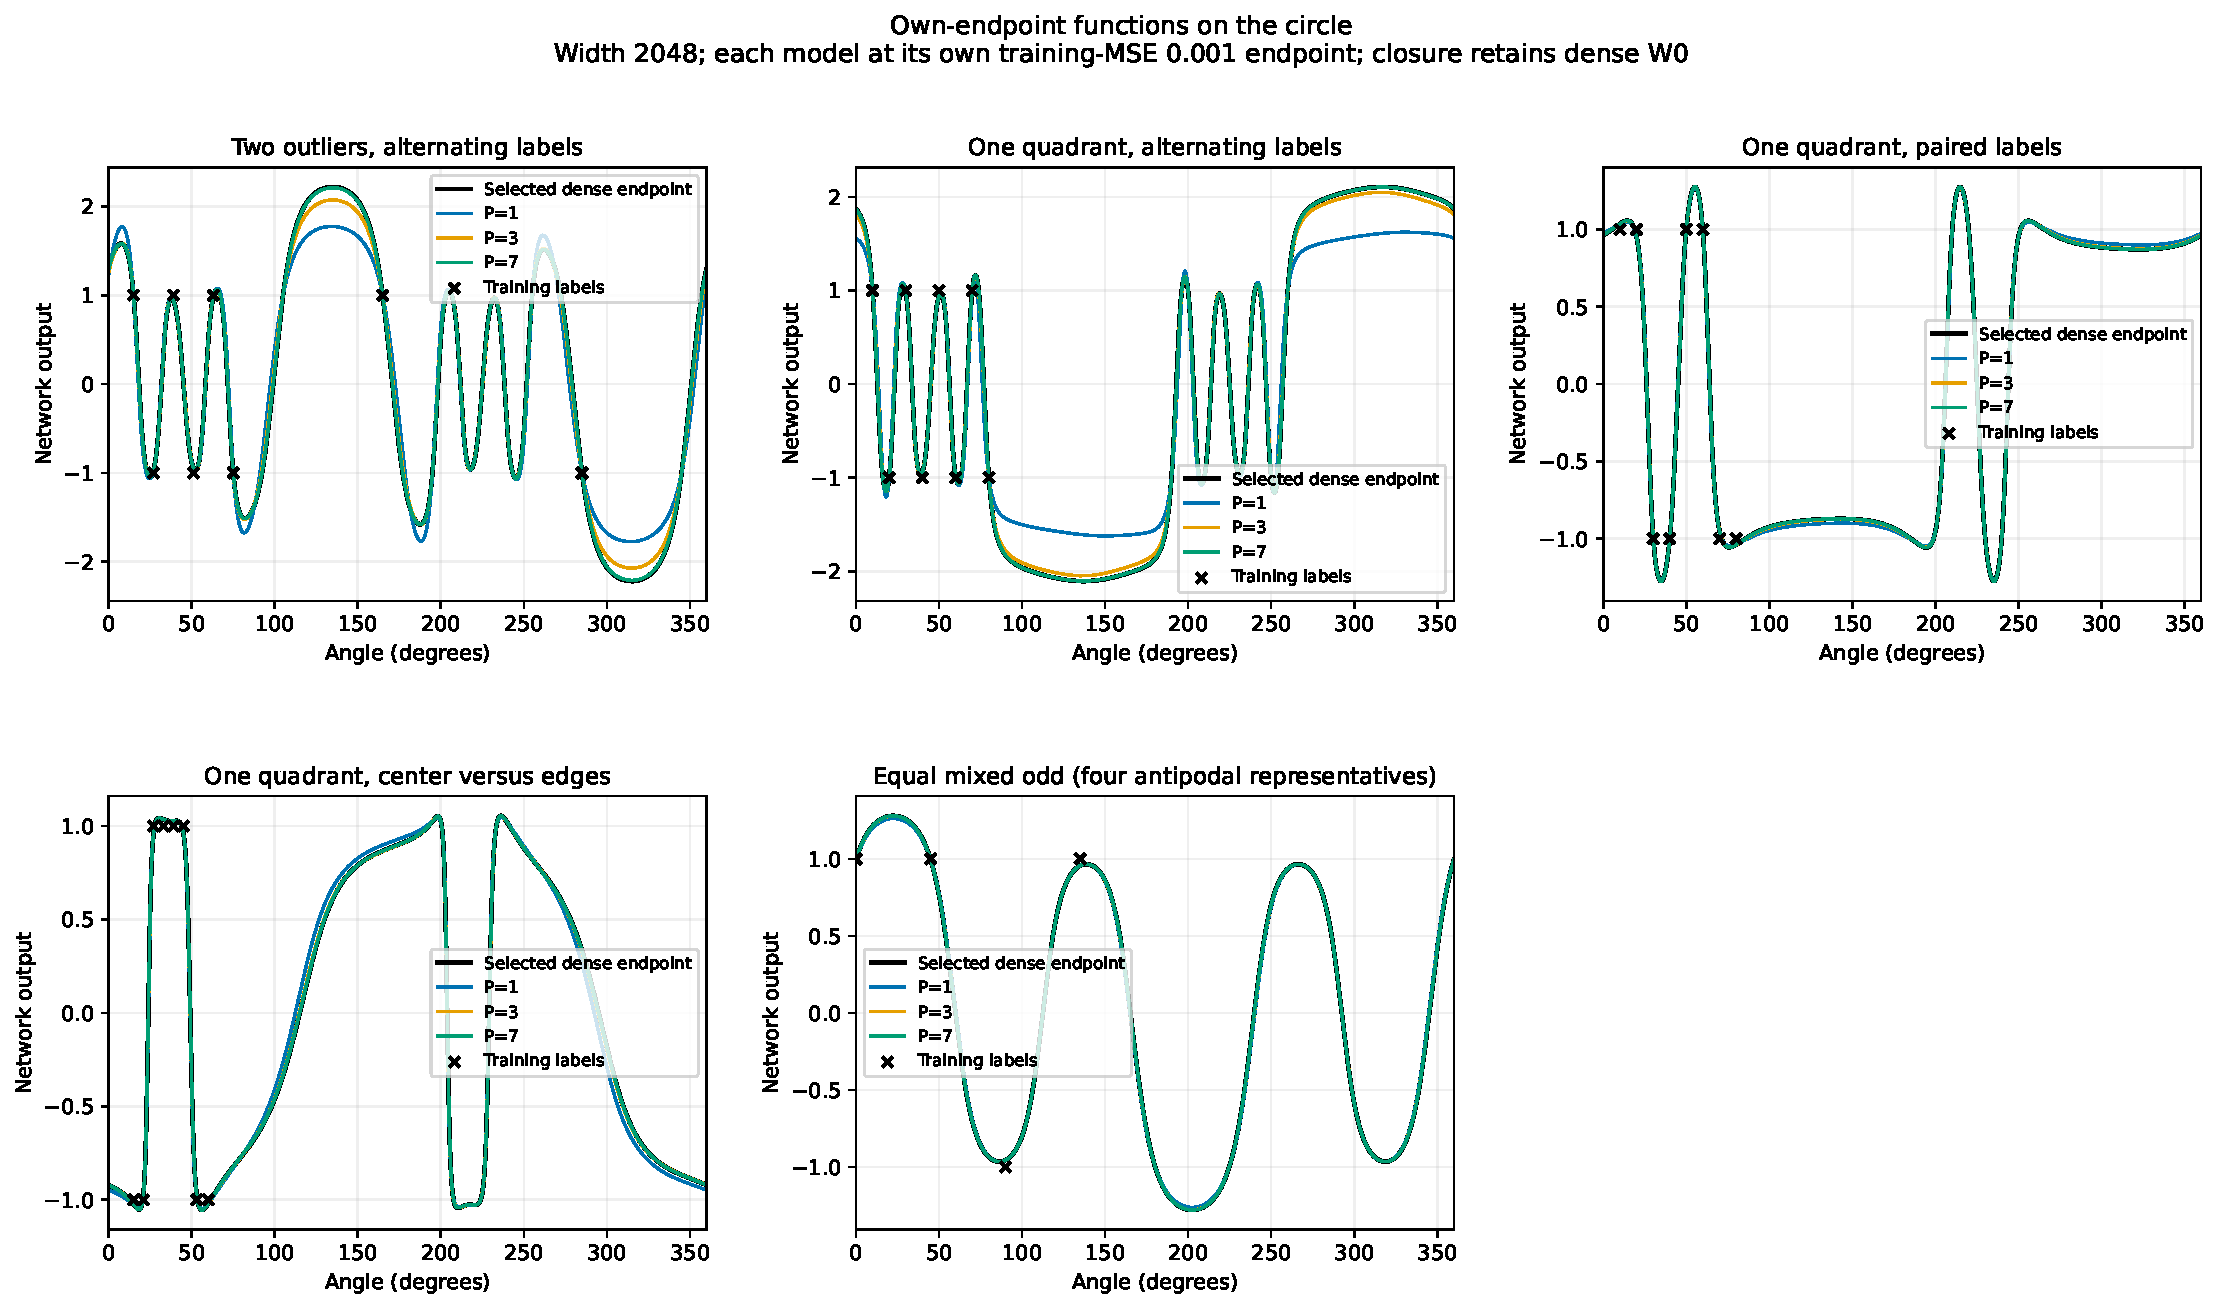
\includegraphics[width=\linewidth]{figures/circle_endpoint_functions.pdf}
\caption{Dense and activity-clock fitted functions for five circle tasks.
Every model is shown at its own first training-MSE $10^{-3}$ crossing.  The
closure retains the dense initialized middle matrix.  The hard-outlier dense
reference is inherited from the frozen benchmark; the other rows have fresh
references checked within the response-memory study.}
\label{fig:circle-functions}
\end{figure}

Figure~\ref{fig:circle-polar} gives the requested radial view for a fully
in-study fresh-reference task.  Network output is signed, so the plotted radius
is explicitly shifted by two; radial tick labels report the original output.

\begin{figure}[t]
\centering
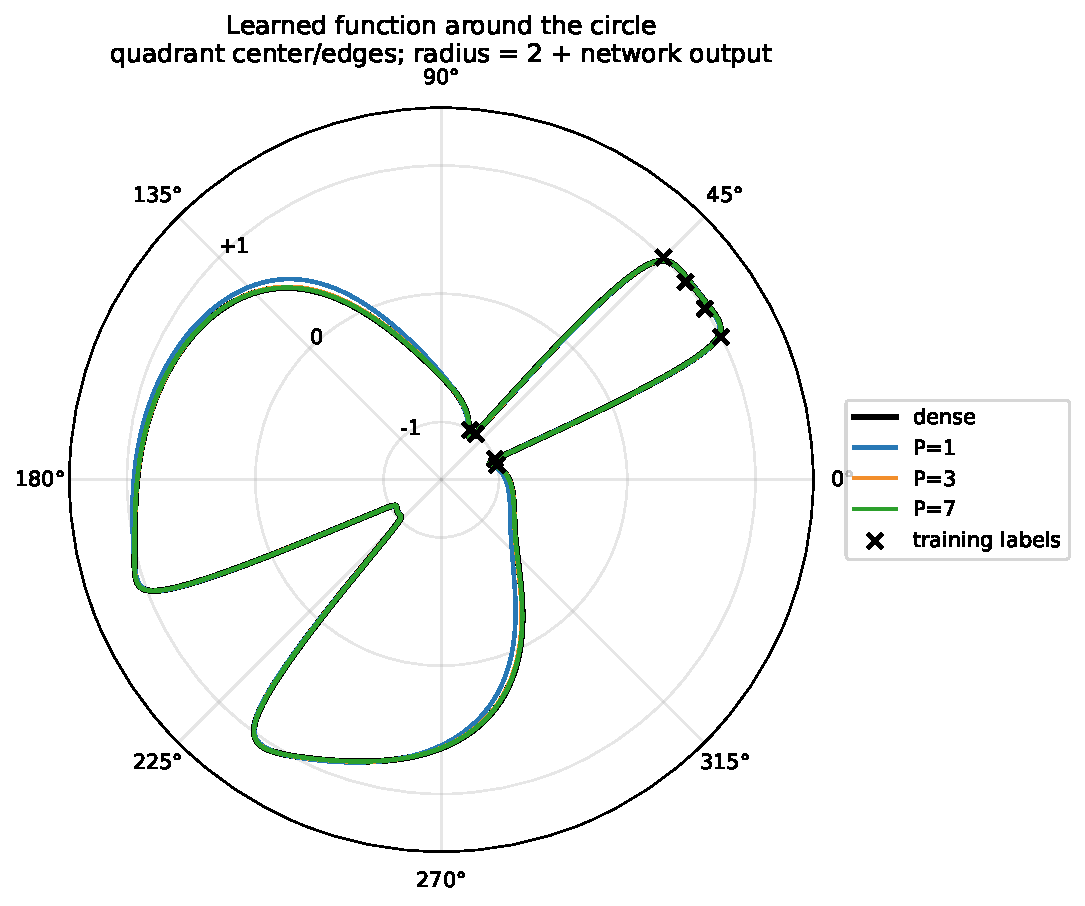
\includegraphics[width=0.72\linewidth]{figures/circle_polar_center_edges.pdf}
\caption{Polar rendering of the quadrant center/edges experiment.  The angle
is the input direction and radius is $2+f(x)$.  Black crosses are training
labels.  The figure is postprocessed from frozen predictions and involves no
new training.}
\label{fig:circle-polar}
\end{figure}

The same construction was tested with three hidden tanh layers of width 4096,
so two dense internal matrices were compressed simultaneously.  Every run
reached MSE $10^{-3}$ and passed the declared numerical gates.  Results in
Table~\ref{tab:deep-circle} show strong improvement over $P=1$, but also two
resolved $P=2$ versus $P=3$ reversals.

\begin{table}[t]
\centering
\small
\caption{Three-hidden-layer circle RMS discrepancy from dense learning at
matched MSE $10^{-3}$.}
\label{tab:deep-circle}
\begin{tabular}{@{}lrrr@{}}
\toprule
Task & $P=1$ & $P=2$ & $P=3$\\
\midrule
Two outliers, alternating & 0.108086 & \textbf{0.023797} & 0.031476\\
Quadrant, alternating & 0.274643 & \textbf{0.028358} & 0.058491\\
Quadrant, paired labels & 0.012186 & 0.003708 & \textbf{0.001215}\\
Quadrant, center/edges & 0.078973 & 0.025702 & \textbf{0.007246}\\
Equal mixed odd & 0.014985 & 0.002412 & \textbf{0.000282}\\
\bottomrule
\end{tabular}
\end{table}

\subsection{Evolving response memory versus fixed or directly trained factors}

The response moments are not a frozen dictionary.  Their columns change with
the current neural responses, and the reconstructed network feeds back into
their derivatives.  In the historical fixed-dictionary experiments, learned
increments were confined to spans chosen at initialization.  Such methods
could fit coefficients but could not acquire new response directions.  On the
same difficult circle functions they were much less efficient in the reported
vector counts.  Those counts do not match total storage because response
memory retains $W_0$.

A cleaner control inside the current study trains a direct factorization
$W=W_0+AB$ by its own Euclidean factor gradient flow, with matched correction
rank and two factor initializations.  Response memory has lower function RMS in
all 29 numerically valid paired cells; 28 differences exceed a factor of two.
At rank 24 on the alternating-outlier task, for example, $P=3$ response memory
has RMS $0.07295$, versus $0.46546$ and $0.46091$ for the two direct-factor
runs.  At rank 56, the response error is $0.00466$ versus $0.51621$ and
$0.25103$.  This rejects the explanation that any low-rank learned correction
would perform equally well under its natural factor flow.  It does not prove
optimality over all low-rank algorithms.

\begin{figure}[t]
\centering
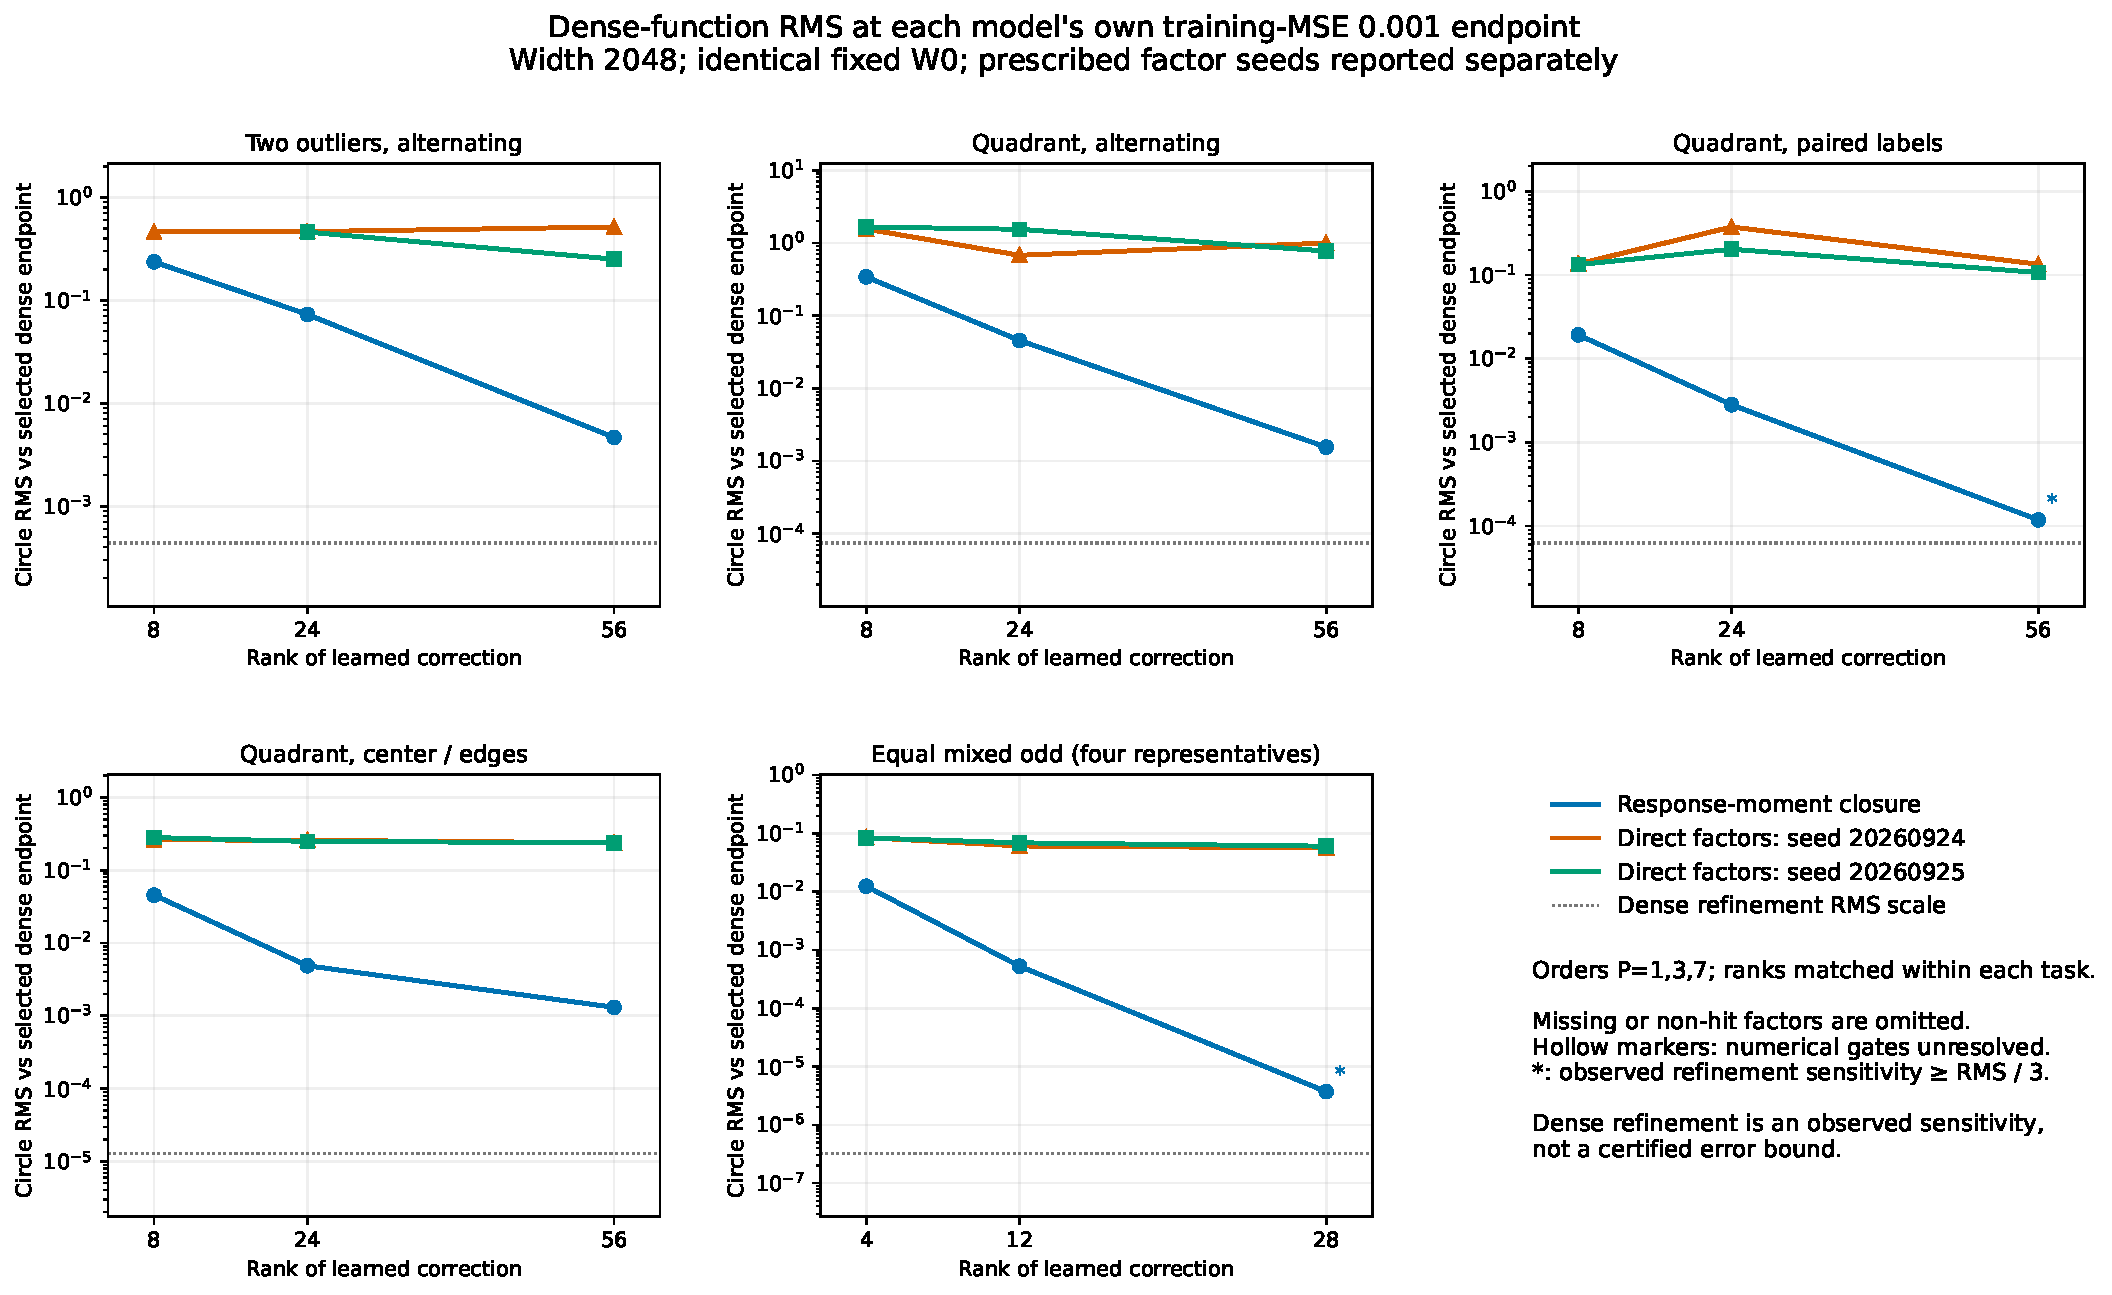
\includegraphics[width=0.88\linewidth]{figures/factor_rms_vs_rank.pdf}
\caption{Response-memory closure versus direct factor-gradient-flow controls
at matched structural rank.  Each model is compared with the same dense fitted
function.  Two factor seeds are shown; one capped factor cell is excluded from
fitted-endpoint comparison.}
\label{fig:factor-control}
\end{figure}

\subsection{MNIST predictions outside the training set}

The MNIST experiment uses digits 3 and 8, 50 training images per class, and all
1984 official-test images of those digits for evaluation.  Inputs are normalized
per image to unit Euclidean norm; no test image enters training, stopping, or
numerical control.  The network has two tanh hidden layers of width 4096.  At
each model's first training-MSE $10^{-3}$ crossing, held-out RMS discrepancy
from dense predictions is
\begin{equation}
 0.00324756\ (P=1),\qquad
 0.00108443\ (P=2),\qquad
 0.00119922\ (P=3).
\end{equation}
All declared refinement gates pass.  The small $P=3$ worsening relative to
$P=2$ is resolved under the frozen diagnostic rule.  All models have the same
held-out classification accuracy, but prediction agreement in
Figure~\ref{fig:mnist} is the relevant closure evidence.

\begin{figure}[t]
\centering
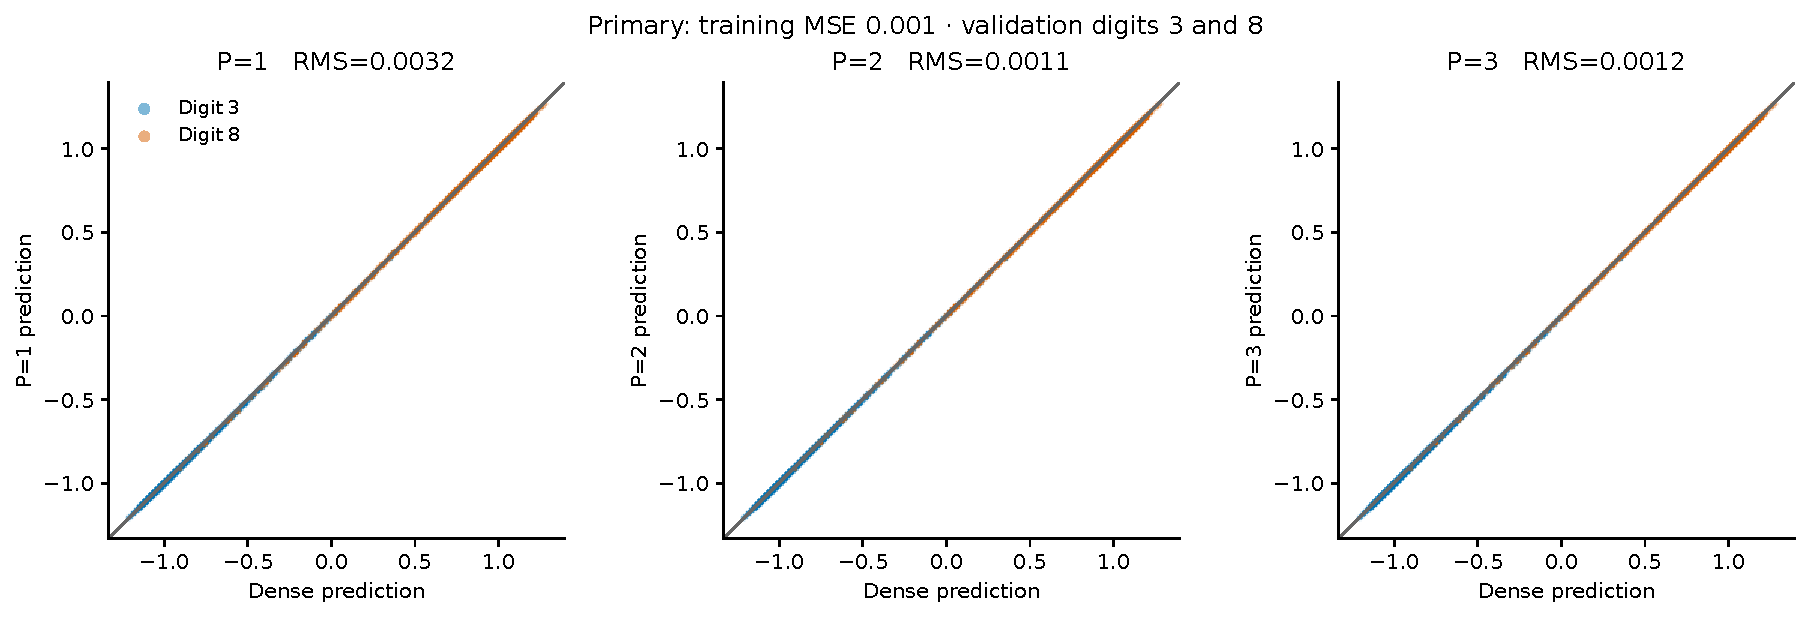
\includegraphics[width=\linewidth]{figures/mnist100_scatter.pdf}
\caption{Held-out closure predictions against dense predictions on 1984 MNIST
3/8 test images.  Models stop at their own training-MSE $10^{-3}$ endpoint.
The correction-rank bounds are 100, 200, and 300 for $P=1,2,3$.}
\label{fig:mnist}
\end{figure}

The history factors occupy $6.25$, $12.50$, and $18.75$ MiB, while an
unrestricted middle correction has $128$ MiB.  Adding the retained $128$ MiB
initialized matrix makes minimal total closure state slightly larger than the
dense current state.  Finest-tolerance integration took $103.0$ seconds for
dense flow and $139.9$, $149.9$, and $152.3$ seconds for the closures.  Measured
CUDA peaks were lower for the closures, but the experiment does not establish
a hardware-independent speedup.

\subsection{The sharper clock: promise and adverse cases}

The response clock has the stronger asymptotic theorem but need not dominate
at low order.  In a focused width-2048 fixed-step panel, all old- and new-clock
models reached training RMS $0.05$.  On the tanh alternating-quadrant task, the
new clock improves the $P=5$ full-circle discrepancy from $0.00658$ to
$0.00346$.  On GELU alternating outliers it improves old-clock $P=5$
$0.00196$ to $0.00098$.  On GELU alternating quadrant, however, its $P=5$
error is $0.99568$, versus $0.01279$ for the activity clock.  Halving the
maximum step reduces the new-clock error to $0.10313$, revealing substantial
finite-step sensitivity without eliminating the gap.

A broader single-seed response-clock sweep contains 82 activation/depth/task
configurations and 328 fits, each capped at 20 seconds.  Dense flow fits 79
configurations; $P=1,2,3$ fit 70, 67, and 66.  On the same 65 configurations
where all four models fit, median closure--dense test RMS is
$0.03147$, $0.01339$, and $0.00658$.  The largest fitted $P=3$ discrepancies
remain $1.36$, $1.25$, and $0.37$ on three alternating-quadrant cases.  The
panel supports typical improvement with order and documents clear exceptions.
It does not empirically verify an $O(P^{-2})$ rate.

All headline experiments use one initialization, and MNIST uses one selected
training subset.  Numerical refinement differences are sensitivity checks,
not rigorous error bars.  Appendix~\ref{app:experiment-tables} records the full
old/new-clock table and resource accounting used here.


\section{Relation to prior work and remaining limits}
\label{sec:context}

\subsection{Exact wide-network descriptions carry history}

Tensor Programs rigorously identify discrete-time infinite-width
feature-learning limits at each fixed finite training horizon
\citep{yang2021tensor}.  In a generic deep nonlinear network, the exact
construction introduces Gaussian variables, covariances, and transpose
response terms indexed by previous steps.  Yang and Hu describe a generic
quadratic-in-step storage and computation burden for this representation.
Recent work proves rich feature nondegeneracy throughout deep $\mu$P training,
while its recursive state continues to contain historical dependencies
\citep{chen2025global}.  These results establish that the standard exact
representation grows with its horizon; they do not prove that every exact
realization must have growing memory.

Self-consistent neural-network DMFT organizes infinite-width feature learning
through two-time activation, gradient, and causal response kernels
\citep{bordelon2022selfconsistent}.  There are also rigorous DMFT convergence
theorems for random-design high-dimensional first-order methods
\citep{celentano2026highdimensional,gerbelot2024rigorous}.  Those theorems take
sample and ambient dimensions to infinity proportionally while keeping a
finite internal learner dimension; they do not directly identify the
fixed-data, all-hidden-width deep regime here.  It would therefore be wrong to
describe DMFT as uniformly nonrigorous, just as it would be wrong to import a
random-design convergence theorem into this network without checking its
regime.

Rigorous multilayer mean-field limits and finite-width couplings are known
under mean-field parametrizations and paper-specific initialization structures
\citep{nguyen2023rigorous,araujo2019meanfield}.  Earlier measure-gradient-flow
work gives foundational shallow particle limits \citep{chizat2018global,
sirignano2020meanfield}.  Our theorem addresses a different question: it
compresses the learned dense increment along a fixed realized nonlinear
gradient-flow trajectory, then controls the induced feedback error.

\subsection{Polynomial memory and low-rank training}

HiPPO is direct prior art for the central memory mechanism
\citep{gu2020hippo}.  It derives online ODEs for optimal polynomial projections
of a signal history, including expanding-interval Legendre coordinates and
approximation bounds.  We do not claim to introduce online Legendre memory.
The additional ingredients here are the identification of paired
forward/backward neural histories, their reconstruction of every internal
learned matrix, an autonomous self-consistent training loop, and a
finite-horizon stability proof for the perturbed trajectory.

Retaining $W_0$ and representing $W_t-W_0$ in low rank also has precedent.
InRank studies cumulative low-rank updates and proves modewise behavior in a
restricted deep-linear setting \citep{zhao2024inrank}; invariant-subspace
compressions have rigorous deep-linear results
\citep{kwon2024compression,yaras2024compressible}.  The response factors here
are neither assumed to lie in a fixed subspace nor optimized as free low-rank
parameters.  They are causal summaries of the dense update's actual response
sources, and their directions evolve as the network learns.

Among the primary sources reviewed for this draft, we did not find a theorem
with the following conjunction: a fixed-order Legendre closure of coupled
forward/backward response histories for deep nonlinear neural-network gradient
flow, together with a finite-horizon trajectory error bound for the closed
system at fixed finite width.  This is a search-qualified distinction, not an
unconditional priority claim.

\subsection{What the result does and does not compress}

The strongest exact statement is deliberately narrow:
\begin{itemize}[leftmargin=*]
\item $P$ is fixed throughout one closure run, so state does not grow with
      elapsed time.
\item The learned dense correction is replaced by population moment fields and
      has a finite-rank action.
\item The initialized hidden matrices are retained as fixed operators, in both
      forward and transpose orientations.
\item Approximation is global on every prescribed finite horizon after choosing
      sufficiently large $P$; it is not uniform over all $t\ge0$.
\item The theorem is fixed-width.  Corollary~\ref{cor:diagonal} gives a
      width-dependent diagonal bridge, not a fixed-order population theorem.
\end{itemize}

These distinctions explain why the result can be both a real training
compression and an incomplete model compression.  It removes the dense
\emph{moving} internal matrices and unbounded historical state.  It does not
remove the random operator that repeatedly mixes neuron populations.  A future
width-uniform theory must either characterize that reused operator by a causal
population law or prove an effective-rank approximation compatible with both
orientations.

The sample index is another unresolved axis.  Current moving state grows as
$mP$ per layer.  Arbitrary labels preclude a universally sample-independent
exact state even in generic fixed-kernel dynamics.  Structured input laws may
permit a second approximation, such as Fourier--Galerkin compression of the
sample-indexed population fields, but that is separate from the theorem here.

\subsection{Open mathematical and empirical questions}

Several questions remain concrete.

\begin{enumerate}[leftmargin=*]
\item \textbf{Width-uniform estimates.}  The constants in
      Theorem~\ref{thm:main} may depend strongly on $n$.  The Euclidean
      response-arclength clock also scales with the concatenated neuron state.
      A population-normalized clock and width-uniform stability estimate are
      needed for a direct $n\to\infty$ theorem at controlled order.
\item \textbf{All-time stability.}  The current bounds contain finite-horizon
      clock lengths and a Gr\"onwall factor.  A uniform all-time result would
      need finite total activity or a trained propagator whose integrated
      amplification remains bounded.
\item \textbf{Initialized-operator compression.}  Compressing $W_0$ while
      preserving its correlated reuse and its adjoint is essential for a true
      total-memory improvement.  Fresh random redraws do not preserve the
      target dynamics.
\item \textbf{Nonsmooth and normalized networks.}  Exact ReLU, normalization
      layers, biases, convolution, residual connections, stochastic gradients,
      and discrete optimizers require new analysis.  Existing numerical tests
      outside the theorem show both successes and failures.
\item \textbf{Practical clock design.}  The response clock proves a better
      asymptotic order but introduces a Gram system and can behave worse at
      small $P$.  A clock optimized for projection error, numerical
      conditioning, and population scaling remains open.
\item \textbf{Statistical validation.}  The present experiments mostly use one
      initialization and matched-loss endpoints.  Seed distributions,
      continuous-time solver certificates, width trends, and broader tasks are
      needed before making general performance claims.
\end{enumerate}

At a conceptual level, a deterministic population learning law could play a
role analogous to an idealized model of computation: finite networks would be
understood through the ideal law plus a quantitative finite-resource error.
That analogy is a research program rather than a conclusion of this paper.
The response-memory theorem supplies one missing component---a controlled
finite description of learned history at fixed width---while leaving the
operator and population-limit steps visible.



\appendix
\section{Supplementary proofs and explicit constants}
\label{app:proofs}

\subsection{Restricted scalar nonclosure}
\label{app:scalar-no-go}

We prove Proposition~\ref{prop:scalar-no-go} in the contraction class stated
there.  Consider four trainable deep-linear factors $(u,B,R,v)$ and output
\begin{equation}
 f_n=v^\top RBu.
\end{equation}
Width normalizations do not affect the graph argument; they can be absorbed
into width-dependent scalar coefficients.  A complete contraction is encoded
by a typed graph whose tensor slots are paired and summed.  Multiplication of
contractions is disjoint union of graphs.

\begin{lemma}[Stable contraction independence]
Every fixed finite family of pairwise nonisomorphic typed complete-contraction
graphs gives linearly independent contraction polynomials for every
sufficiently large width.
\end{lemma}

\begin{proof}
Treat tensor entries as independent commuting indeterminates.  For every graph
$G$, partition all index assignments according to which index vertices are
equal.  This writes its contraction as
\begin{equation}
 P_G^{(n)}=\sum_\pi I_{G/\pi}^{(n)},
\end{equation}
where $I_H^{(n)}$ sums only injective labelings of the quotient incidence
network $H$.  Once width exceeds the number of vertices of each type, an
injective labeling produces a tensor-entry monomial that records the typed
incidence network.  It occurs in another injective contraction only for an
isomorphic network.  Hence distinct injective contractions are independent.
In a purported relation among the $P_G^{(n)}$, choose a graph with a maximal
number of index vertices.  Its discrete-partition injective term cannot be
cancelled by any proper quotient, which has fewer vertices, or by a
nonisomorphic graph of the same size.  Descending in vertex count proves that
all coefficients vanish.
\end{proof}

Let $A=RB$ and $H=A^\top A$.  Retain only differentiation of the endpoint
factors in the feature derivative:
\begin{equation}
 \mathcal D_{0,n}v=Au,qquad
 \mathcal D_{0,n}u=A^\top v,qquad
 \mathcal D_{0,n}A=0.
\end{equation}
For $j\ge0$ put
\begin{equation}
 U_j=v^\top AH^ju,quad
 X_j=u^\top H^{j+1}u,quad
 Y_j=v^\top(AA^\top)^{j+1}v.
\end{equation}
Direct differentiation gives
\begin{equation}
 \mathcal D_{0,n}U_j=X_j+Y_j,qquad
 \mathcal D_{0,n}X_j=\mathcal D_{0,n}Y_j=2U_{j+1}.
\end{equation}
Therefore, for $j\ge1$,
\begin{equation}
 \mathcal D_{0,n}^{,2j-1}f_n
 =4^{j-1}\left[u^\top H^ju+v^\top(AA^\top)^jv\right].
 \label{eq:no-go-derivatives}
\end{equation}
In the full feature derivative, every tensor replacement and product-rule
coefficient is nonnegative.  Hence the connected contraction
\begin{equation}
 \Gamma_j=u^\top(B^\top R^\top RB)^ju
\end{equation}
appears with positive coefficient in
$\mathcal D_n^{,2j-1}f_n$.  Its tensor degree is $4j+2$, so the connected
graph types $\Gamma_j$ have unbounded complexity.

Now suppose a fixed encoder uses contractions from a finite bounded-degree
alphabet $\mathcal S$ and evolves by a polynomial autonomous ODE with a
polynomial output readout.  Every time derivative of the output obtained from
that ODE is a polynomial in encoder coordinates.  Its contraction graph is
therefore a disjoint union of connected components from $\mathcal S$.  Choose
$j$ so that $\Gamma_j\notin\mathcal S$.  Equation
\eqref{eq:no-go-derivatives} and stable independence contradict the equality
between the true and encoded $(2j-1)$st output derivatives.  An identity on a
nonempty open state set is a polynomial identity, so the same coefficient
comparison applies globally.

For an analytic finite-jet closure near zero, scale every factor by a common
$\lambda$ and compare the homogeneous Taylor coefficient of the degree of
$\Gamma_j$.  At any fixed power of $\lambda$, only finitely many Taylor
monomials contribute, and their connected components still lie in
$\mathcal S$.  The same contradiction follows.

For squared-loss physical flow, the vector field is a scalar multiple of the
feature field,
\begin{equation}
 \mathcal X_n=-2\kappa(f_n-y)\mathcal D_n.
\end{equation}
If $y\ne0$, the lowest-degree part of
$\mathcal X_n^kf_n$ is $(2\kappa y)^k\mathcal D_n^kf_n$.  If $y=0$, positivity
of graph coefficients shows that the relevant derivative contains a positive
multiple of $f_n^k\mathcal D_n^kf_n$.  In either case a connected component
$\Gamma_j$ outside $\mathcal S$ remains, completing the proof.

The bounded-degree, state-universal, and regular-readout assumptions are
essential.  An unrestricted field can encode the entire future output germ,
and the proposition makes no claim about such oracle encodings or about one
special initialized trajectory.

\subsection{Explicit constants for Theorem~\ref{thm:main}}
\label{app:constants}

This subsection records one concrete choice of the finite constants used in
the main proof.  It also makes clear where width, depth, and horizon enter.

Let
\begin{equation}
 R=\norm{\theta_0}+\sqrt{nT}\rho_0+1,qquad
 \cB=\{\theta:\norm\theta\le R\},qquad \rho_0=\rho(0)>0.
\end{equation}
Put $X=\max_a\norm{u_a}$, $M_0=X$, and recursively define
\begin{align}
s_\ell&=\sup_{|z|\le RM_{\ell-1}}|\phi_\ell'(z)|,
&M_\ell&=\sqrt n\sup_{|z|\le RM_{\ell-1}}|\phi_\ell(z)|,\nonumber\\
B_L&=Rs_L,
&B_\ell&=s_\ell R B_{\ell+1}\quad(\ell<L).
\label{eq:explicit-response-bounds}
\end{align}
These give $\norm{h_{\ell,a}}\le M_\ell$ and
$\norm{\delta_{\ell,a}}\le B_\ell$ on $\cB$.  Let
\begin{align}
Y&=\left(m^{-1}\sum_a y_a^2\right)^{1/2},&
q&=RM_L/n+Y,&S&=Tq,&\ell_T&=1+S,\nonumber\\
v_1&=2B_1X,&
v_\ell&=2B_\ell M_{\ell-1}/n\quad(\ell\ge2),&
v_w&=2M_L,\nonumber\\
V&=\left(v_1^2+\sum_{\ell=2}^Lv_\ell^2+v_w^2\right)^{1/2},
\label{eq:explicit-V}
\end{align}
and
\begin{equation}
 c_f=\frac1n\left[(B_1X)^2+
 \sum_{\ell=2}^L(B_\ell M_{\ell-1})^2+M_L^2\right]^{1/2}.
 \label{eq:explicit-cf}
\end{equation}
Sample Cauchy--Schwarz gives $\norm F\le V\rho$ and the gradient of
each output is bounded by $c_f$.  A finite Lipschitz constant $K$ for $F$ on
the compact convex ball follows from the local Lipschitz activation bounds.

For Variant A, a concrete order-independent derivative recursion is
\begin{align}
\overline Z_1&=S(s_1v_1X)^2,\nonumber\\
\overline Z_\ell&=3s_\ell^2\left[
 S v_\ell^2M_{\ell-1}^2+
 \left(R^2+\frac{2B_\ell^2\ell_T^2M_{\ell-1}^2}{n^2}\right)
 \overline Z_{\ell-1}\right].
\label{eq:explicit-Z}
\end{align}
The derivation is exactly \eqref{eq:A-e}--\eqref{eq:A-chain}, using
$\norm{x+y+z}^2\le3(\norm x^2+\norm y^2+\norm z^2)$.  One may take
\begin{equation}
 \Gamma_A=\frac{\ell_T}{n}\sum_{\ell=2}^L
 B_\ell\sqrt{S\overline Z_{\ell-1}},qquad
 C_A(T)=\Gamma_Ae^{KT}.
 \label{eq:explicit-GammaA}
\end{equation}

For Variant B, define
\begin{equation}
 Q=m\sum_{\ell=2}^L(M_{\ell-1}^2+B_\ell^2),qquad
 C_0=\frac{\ell_TQ}{nm}.
\end{equation}
On the stopped region $\rho\ge\mu/2$, let $J$ be a bound for the derivative
of the current response map $\theta\mapsto\Psi(\theta)$.  Then
\begin{equation}
 \Lambda_T=\ell_T+J(VS+C_0),qquad
 \Gamma_B=\frac{\Lambda_T^2(\Lambda_T-1)}{4nm},qquad
 C_B(T)=\Gamma_Be^{KT}.
 \label{eq:explicit-GammaB}
\end{equation}
Choose $P_A(T)$ so
$\Gamma_Ae^{KT}/\sqrt{P(P+1)}\le1/2$.  Choose $P_B(T)$ so both
\begin{equation}
 \frac{\Gamma_Be^{KT}}{P(P+1)}\le\frac12,
 \qquad
 c_f\frac{\Gamma_Be^{KT}}{P(P+1)}\le\frac\mu4.
\end{equation}
These choices close the first-exit arguments.

\subsection{All orders for bounded activations}

Suppose $\norm{\phi_\ell}_\infty$ and
$\norm{\phi_\ell'}_\infty$ are finite.  Put
$M_\ell=\sqrt n\norm{\phi_\ell}_\infty$ and
$s_\ell=\norm{\phi_\ell'}_\infty$.  The readout equation gives the exact
estimate
\begin{equation}
 \frac\od{\od t}\norm w^2
 =-\frac{4n}{m}\sum_a(f_a-y_a)f_a
 \le nY^2.
\end{equation}
Thus $B_w=(\norm{w_0}^2+nY^2T)^{1/2}$ bounds the readout.  Let
\begin{equation}
 q=B_wM_L/n+Y,qquad S=Tq,qquad \ell_T=1+S,qquad B_L=B_ws_L.
\end{equation}
Proceed downward from layer $L$ to layer two:
\begin{equation}
 D_\ell=\norm{W_{\ell,0}}_F+
 \frac{2\ell_TB_\ell M_{\ell-1}}n,qquad
 B_{\ell-1}=s_{\ell-1}D_\ell B_\ell.
 \label{eq:bounded-downward}
\end{equation}
Projection contraction bounds the Variant A learned increment by the second
term in $D_\ell$; the dense increment is no larger.  Hence
$\norm{\what W_\ell}_F\le D_\ell$, and the backward recurrence gives the next
$B_{\ell-1}$.  Finally,
\begin{equation}
 \norm{W_1(t)}_F\le\norm{W_{1,0}}_F+2SB_1X.
\end{equation}
All physical bounds are independent of $P$.  At fixed order, the moment
integrals are bounded because $1\le\tau\le\ell_T$ and every history is
bounded.  Standard ODE continuation gives global physical-time existence for
every $P$.  Repeating \eqref{eq:explicit-Z} with $D_\ell$ in place of $R$
gives \eqref{eq:old-rate} for all orders.


\section{Supplementary empirical tables}
\label{app:experiment-tables}

\subsection{Full focused old/new-clock comparison}

Table~\ref{tab:clock-full} reports the focused width-2048 panel at each model's
own first training-RMS $0.05$ endpoint.  The maximum Euler step is $1/64$,
TF32 is disabled, and every displayed model reaches the training target.

\begin{table}[h]
\centering
\scriptsize
\caption{Full-circle RMS from a freshly fitted dense reference.  ``Old'' is
the activity clock and ``New'' is the response-arclength clock.}
\label{tab:clock-full}
\begin{tabular}{@{}lllrrrrr@{}}
\toprule
Activation/depth & Task & Clock & P1 & P2 & P3 & P4 & P5\\
\midrule
tanh/2 & Alternating outliers & Old & .07250 & .04009 & .01674 & .00524 & .00123\\
tanh/2 & Alternating outliers & New & .07018 & .04901 & .01323 & .00786 & .00324\\
tanh/2 & Alternating quadrant & Old & .05417 & .06186 & .02388 & .00818 & .00658\\
tanh/2 & Alternating quadrant & New & .06552 & .09918 & .01283 & .00591 & .00346\\
tanh/2 & Paired quadrant & Old & .00566 & .00135 & .00056 & .00022 & .00007\\
tanh/2 & Paired quadrant & New & .00833 & .00124 & .00111 & .00032 & .00019\\
GELU/3 & Alternating outliers & Old & .44504 & .07570 & .00549 & .00207 & .00196\\
GELU/3 & Alternating outliers & New & .45472 & .11902 & .04500 & .00679 & .00098\\
GELU/3 & Alternating quadrant & Old & 2.98734 & .20941 & .11963 & .01469 & .01279\\
GELU/3 & Alternating quadrant & New & 3.06966 & 2.69207 & 1.24526 & 1.21472 & .99568\\
GELU/3 & Paired quadrant & Old & .08807 & .00574 & .00443 & .00149 & .00077\\
GELU/3 & Paired quadrant & New & .11162 & .00674 & .00157 & .00206 & .00016\\
\bottomrule
\end{tabular}
\end{table}

For the adverse GELU alternating-quadrant case, halving the maximum step to
$1/128$ gives
\begin{align*}
\text{old clock: }&(2.99053,\ 0.21233,\ 0.11999,\ 0.02364,\ 0.02150),\\
\text{new clock: }&(3.07505,\ 2.90895,\ 0.11200,\ 0.22258,\ 0.10313).
\end{align*}
This is an endpoint numerical sensitivity result, not a
continuous-gradient-flow certificate.

\subsection{Measured state and runtime examples}

\begin{table}[h]
\centering
\scriptsize
\caption{Representative measured resources.  ``Total'' adds the fixed
initialized internal matrix or matrices to moving state and excludes solver
workspace.  CUDA peak includes implementation workspace.}
\label{tab:resource-full}
\begin{tabular}{@{}llrrrr@{}}
\toprule
Experiment & Model & Moving MiB & Moving+fixed MiB & CUDA peak MiB & Integration s\\
\midrule
MNIST100, $n=4096$ & Dense & 152.531 & 152.531 & 1941.881 & 102.976\\
& P1 & 30.781 & 158.781 & 544.266 & 139.893\\
& P2 & 37.031 & 165.031 & 603.141 & 149.922\\
& P3 & 43.281 & 171.281 & 654.391 & 152.269\\
\midrule
Deep circle, $n=4096$ & Dense & 256.094 & 256.094 & 2592.9--2849.0 & task-dependent\\
& P1 & 1.094 & 257.094 & 432.063 & slower than dense\\
& P2 & 2.094 & 258.094 & 432.063 & slower than dense\\
& P3 & 3.094 & 259.094 & 432.063 & slower than dense\\
\bottomrule
\end{tabular}
\end{table}

The measured peak reduction comes from the particular solver representation;
the mathematical state ledger shows no total-state reduction once $W_0$ is
counted.  The closure's durable advantage in the present form is that the
learned moving correction and stored history are low rank and independent of
elapsed training time.


\bibliographystyle{plainnat}
\bibliography{references}
\end{document}
